
\ref{non-crime-no-timeseries-result}同様に予測結果を示す.

2014年に実際に起った強盗犯罪の発生地点とそれに基づいた実際のリスクマップを
図\ref{fig:add-crime-timeseries-actual-risk}に示す.
DFによるリスクマップを図\ref{fig:add-crime-timeseries-df-risk}に,
CFによるリスクマップを図\ref{fig:add-crime-timeseries-cf-risk}に示す.
NEによるリスクマップを図\ref{fig:add-crime-timeseries-ne-risk}に,
LDによるリスクマップを図\ref{fig:add-crime-timeseries-ld-risk}に,
GFによるリスクマップを図\ref{fig:add-crime-timeseries-gf-risk}に,
TGによるリスクマップを図\ref{fig:add-crime-timeseries-tg-risk}に,
GF+TGによるリスクマップを図\ref{fig:add-crime-timeseries-gf-tg-risk}に示す.
\ref{non-crime-no-timeseries-result}同様に,
実際のリスクマップと比べて,離散型特徴量によるリスクマップでは高い空間相関を持つが,
連続型特徴量によるリスクマップは空間相関が削減された.

また,
4カテゴリーの混同行列を図\ref{fig:add-crime-timeseries-4cm}に,
2カテゴリーの混同行列を図\ref{fig:add-crime-timeseries-2cm}に,
各モデルによるFP・FNのグリッドセルを
図\ref{fig:add-crime-timeseries-df-fnp}から
図\ref{fig:add-crime-timeseries-gf-tg-fnp}に示した.

%------------------------------------------
% risk map
%------------------------------------------
\begin{figure}
  \centering % 図を中央寄せにする
  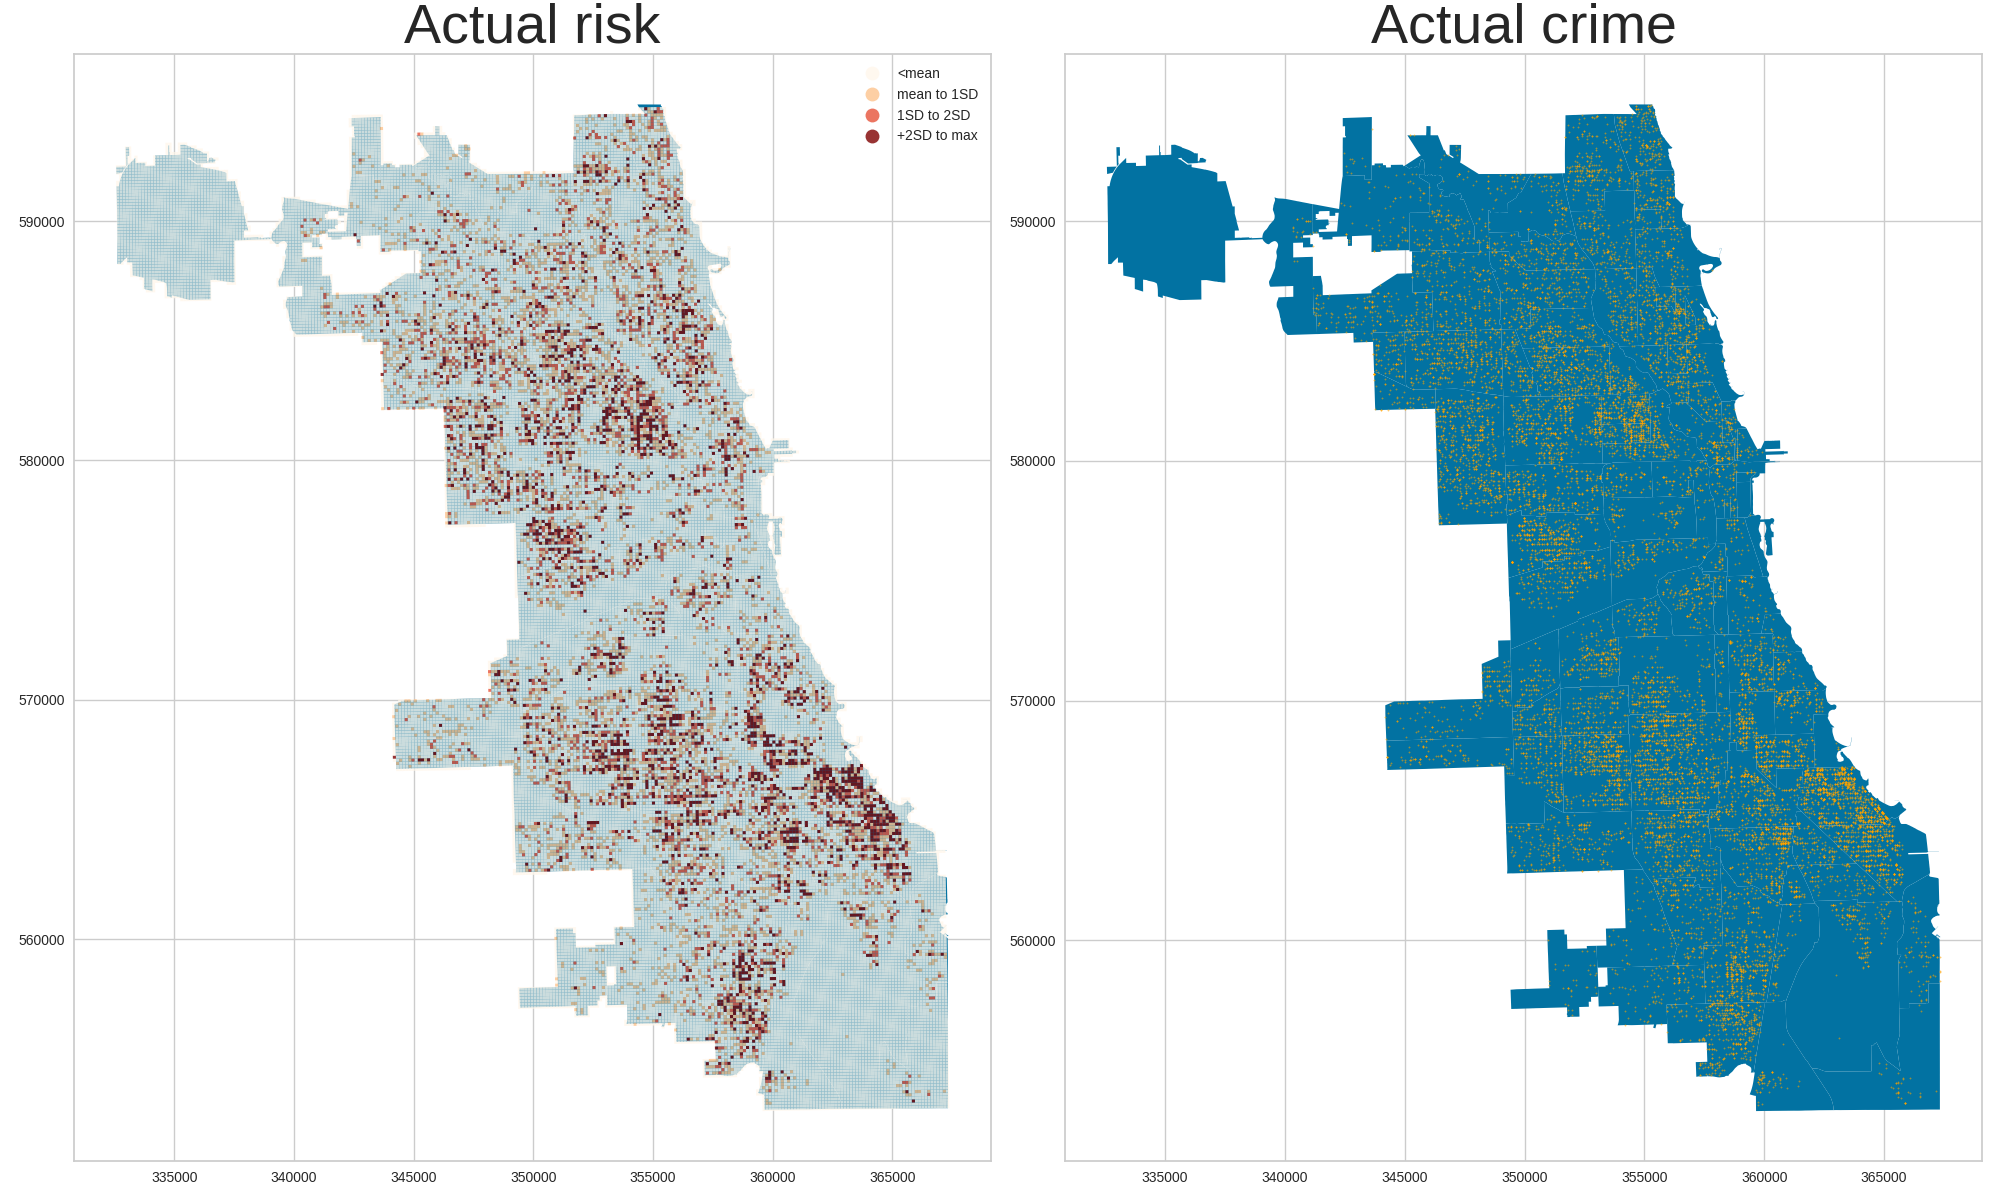
\includegraphics[scale=0.25]{./util-fig/actual_risk_point_map.png}
  \caption{左:実際のリスクマップ 右:実際の強盗犯罪発生地点}
  \label{fig:add-crime-timeseries-actual-risk}
\end{figure}

\begin{figure}
  \centering % 図を中央寄せにする
  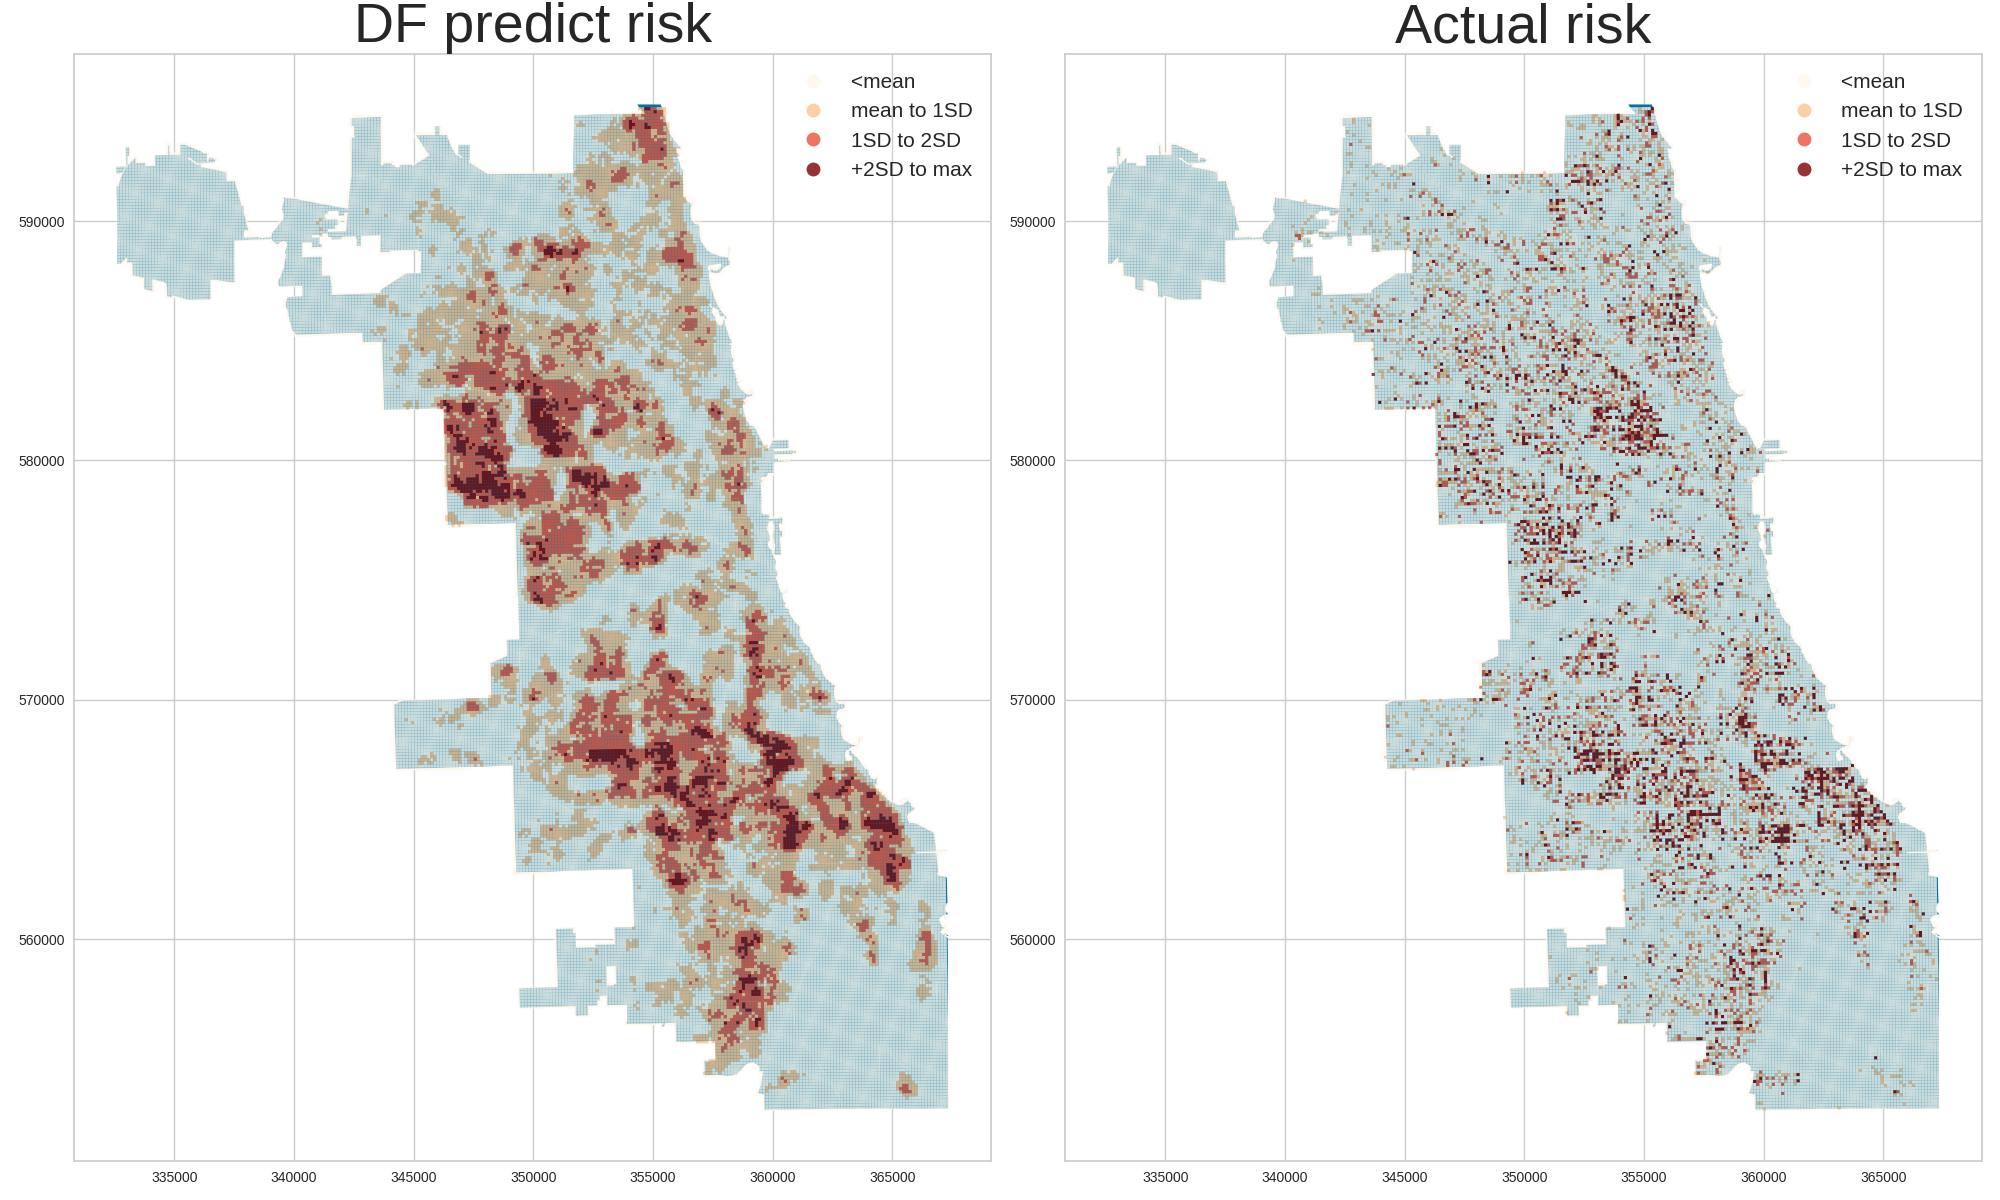
\includegraphics[scale=0.25]{./add-crime-timeseries-fig/DF_riskmap.png}
  \caption{左:DFによるリスクマップ 右:実際のリスクマップ}
  \label{fig:add-crime-timeseries-df-risk}
\end{figure}

\begin{figure}
  \centering % 図を中央寄せにする
  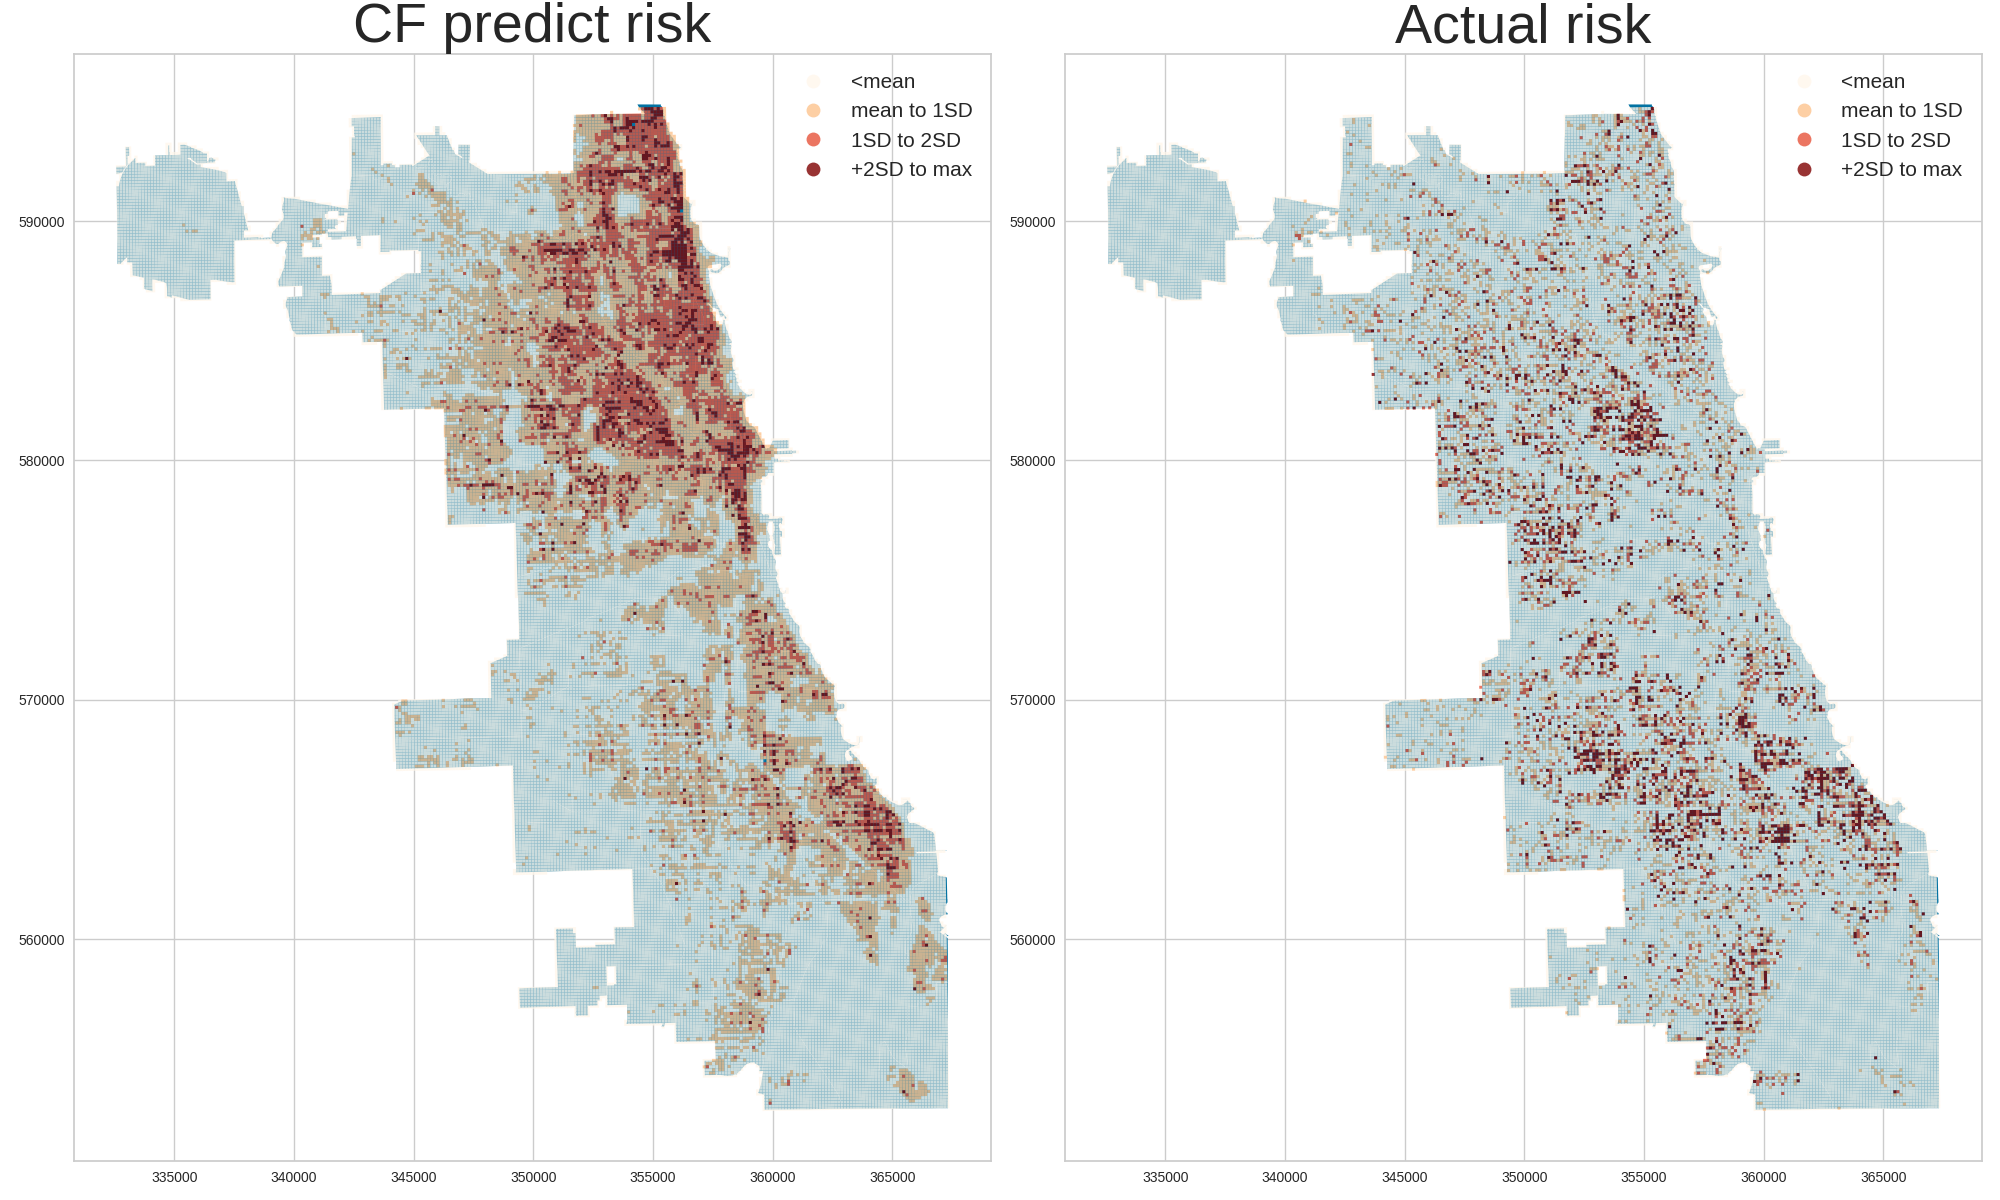
\includegraphics[scale=0.25]{./add-crime-timeseries-fig/CF_riskmap.png}
  \caption{左:CFによるリスクマップ 右:実際のリスクマップ}
  \label{fig:add-crime-timeseries-cf-risk}
\end{figure}

\begin{figure}
  \centering % 図を中央寄せにする
  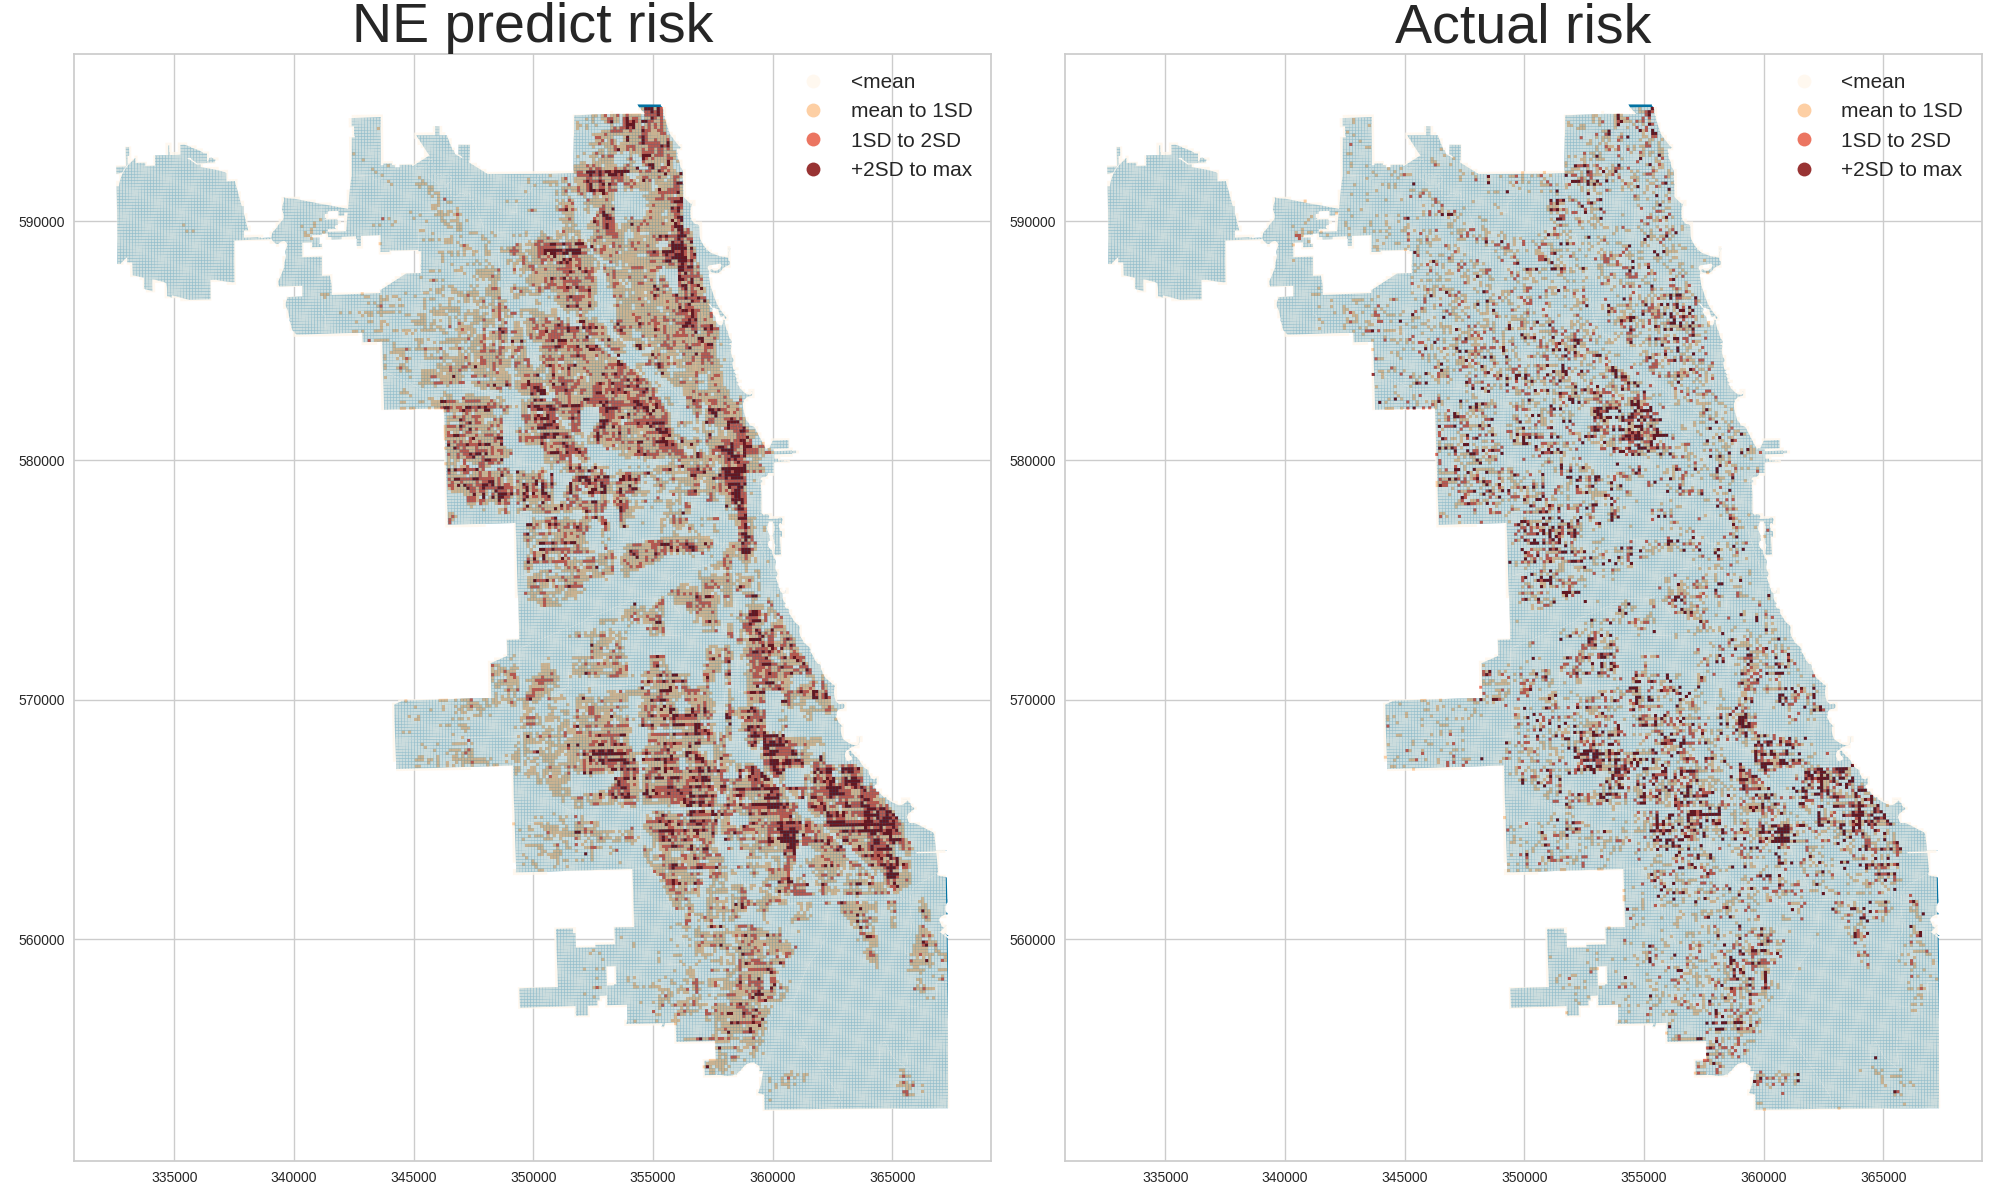
\includegraphics[scale=0.25]{./add-crime-timeseries-fig/NE_riskmap.png}
  \caption{左:NEによるリスクマップ 右:実際のリスクマップ}
  \label{fig:add-crime-timeseries-ne-risk}
\end{figure}

\begin{figure}
  \centering % 図を中央寄せにする
  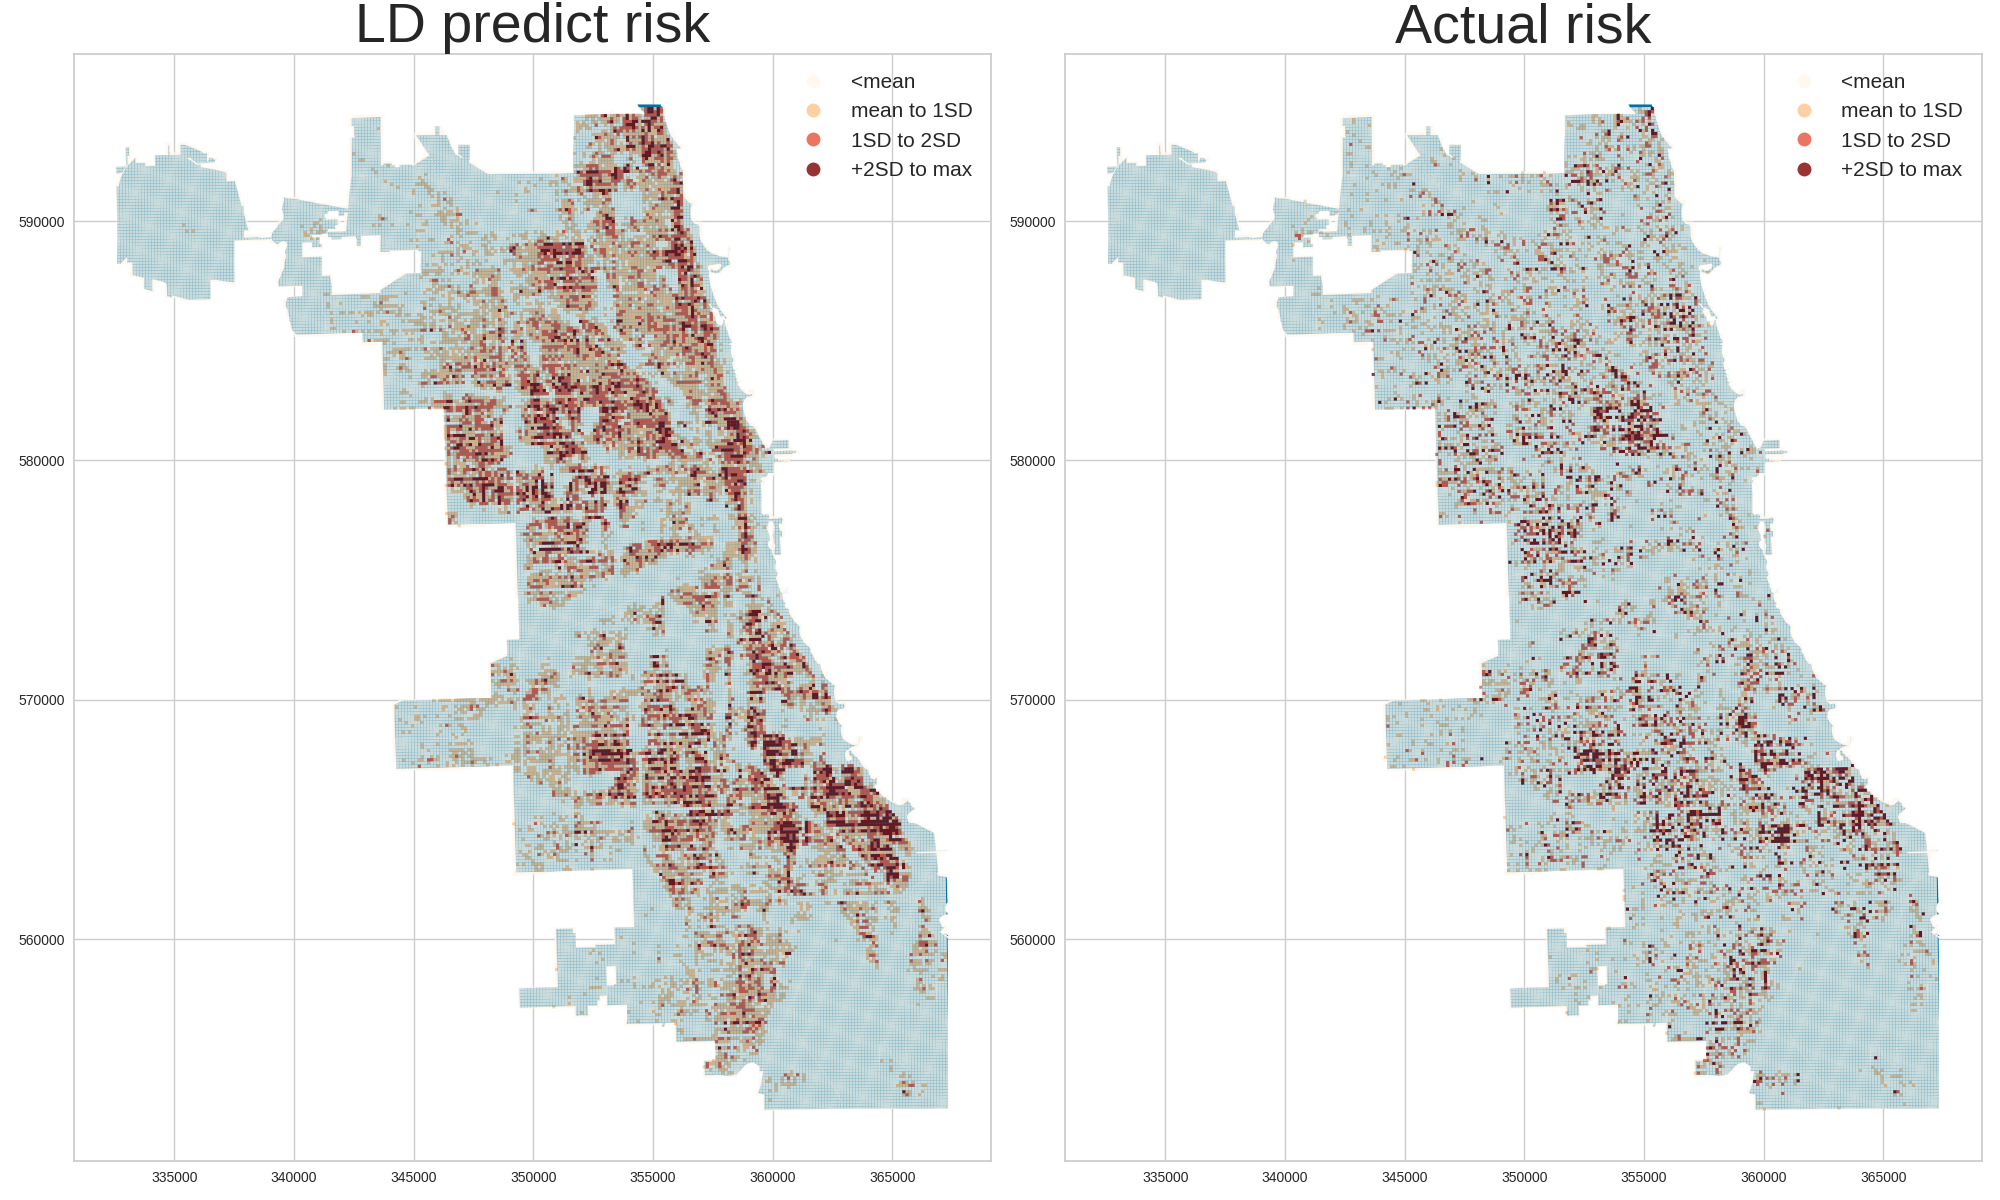
\includegraphics[scale=0.25]{./add-crime-timeseries-fig/LD_riskmap.png}
  \caption{左:LDによるリスクマップ 右:実際のリスクマップ}
  \label{fig:add-crime-timeseries-ld-risk}
\end{figure}

\begin{figure}
  \centering % 図を中央寄せにする
  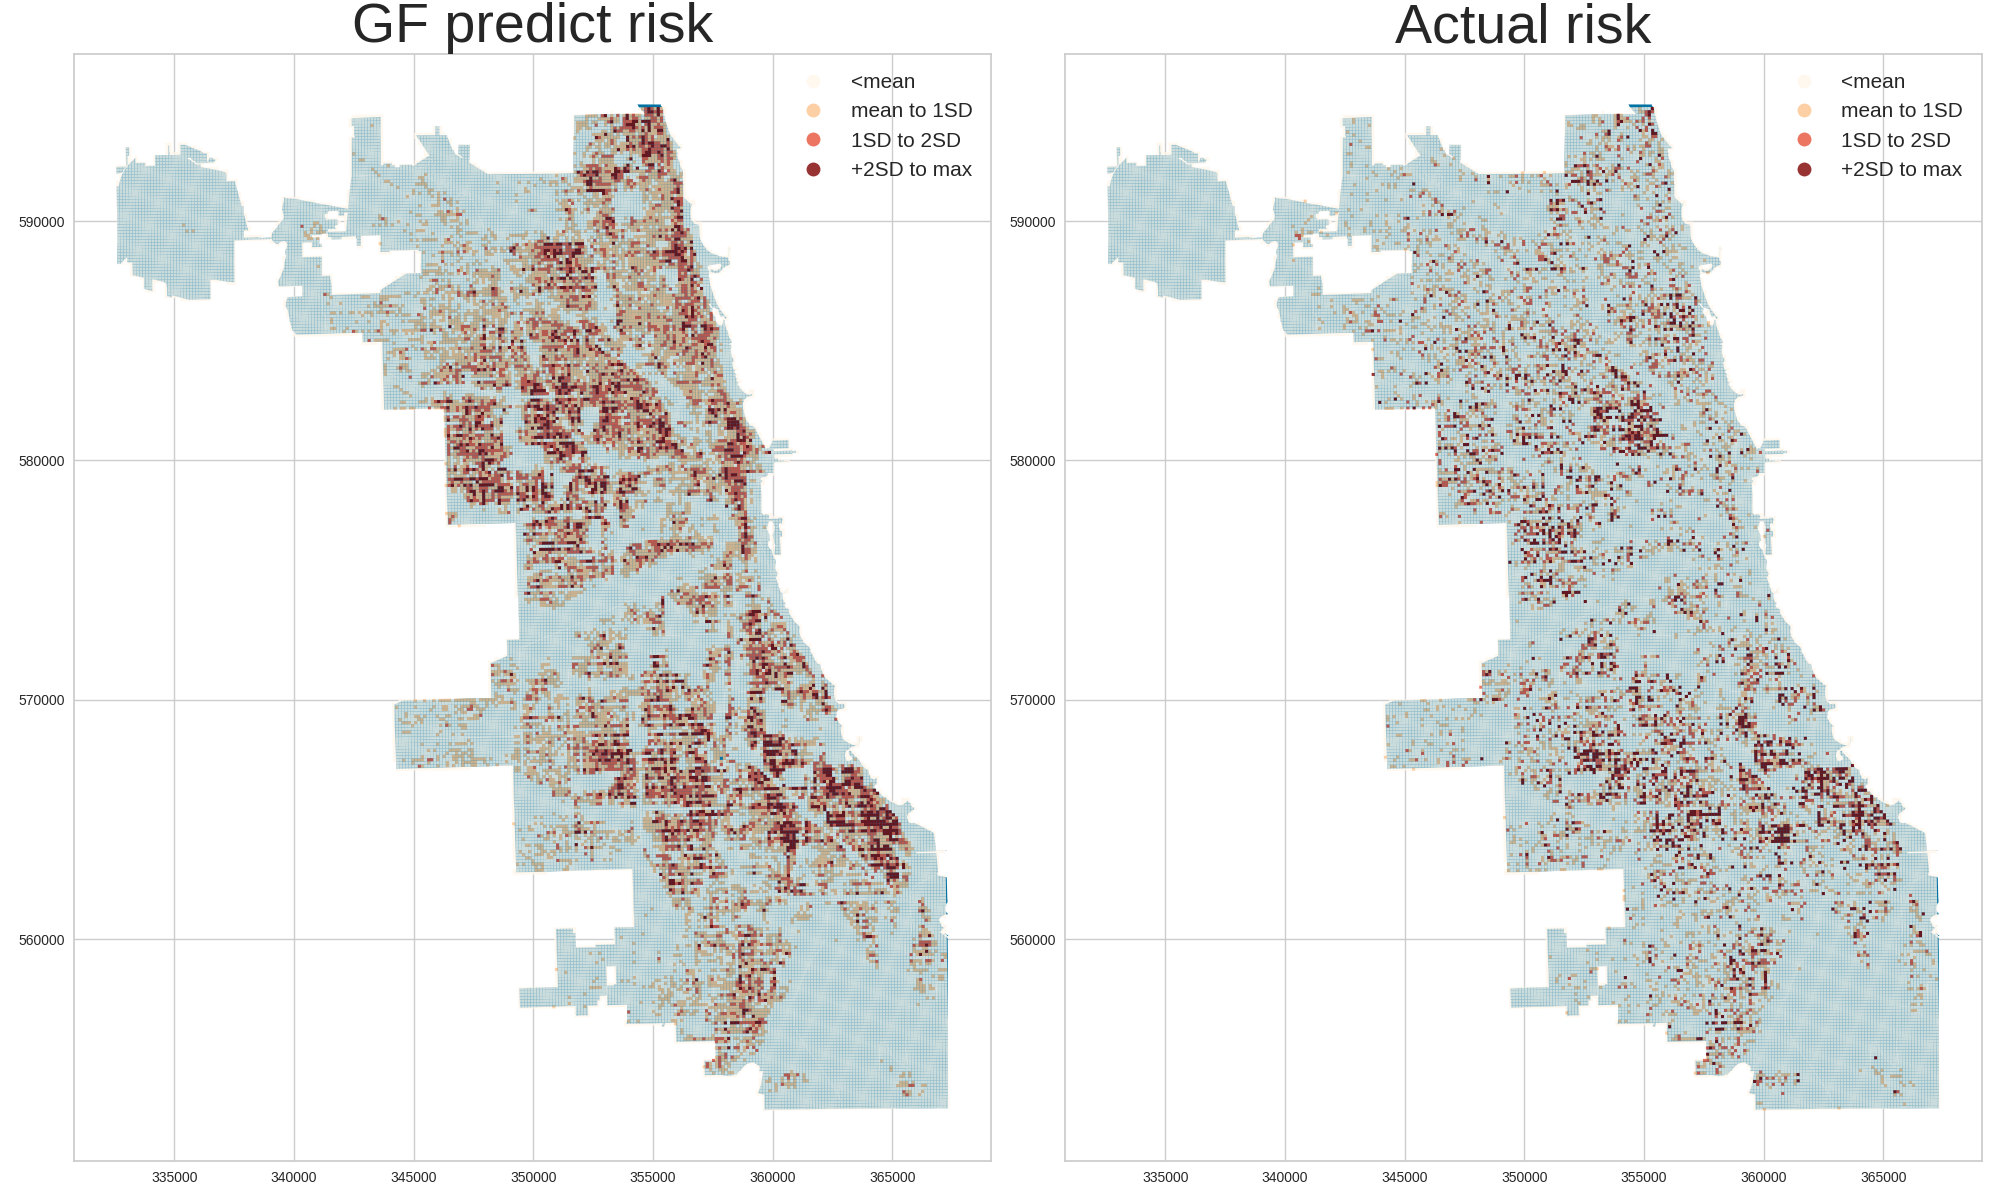
\includegraphics[scale=0.25]{./add-crime-timeseries-fig/GF_riskmap.png}
  \caption{左:GFによるリスクマップ 右:実際のリスクマップ}
  \label{fig:add-crime-timeseries-gf-risk}
\end{figure}

\begin{figure}
  \centering % 図を中央寄せにする
  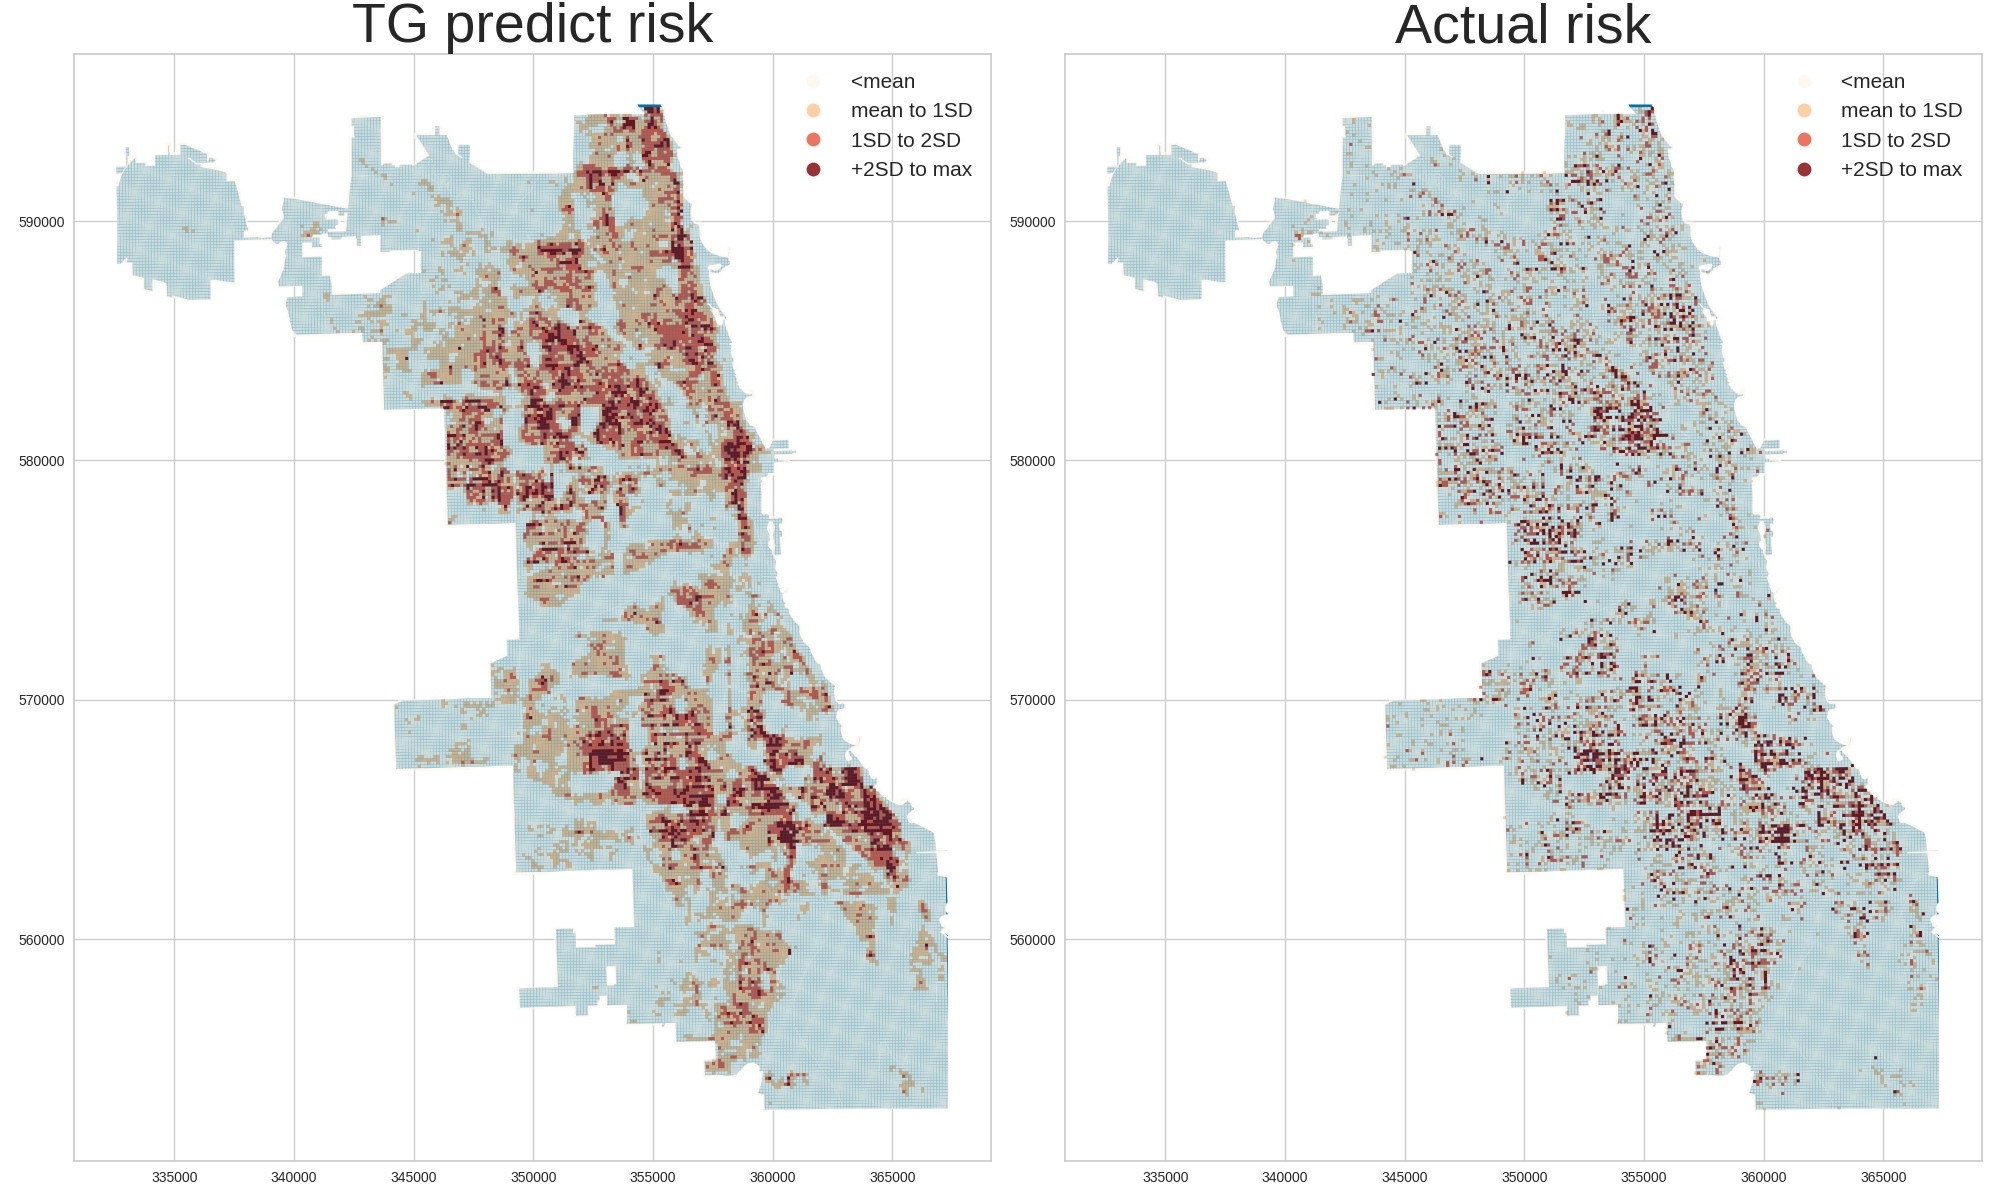
\includegraphics[scale=0.25]{./add-crime-timeseries-fig/TG_riskmap.png}
  \caption{左:TGによるリスクマップ 右:実際のリスクマップ}
  \label{fig:add-crime-timeseries-tg-risk}
\end{figure}

\begin{figure}
  \centering % 図を中央寄せにする
  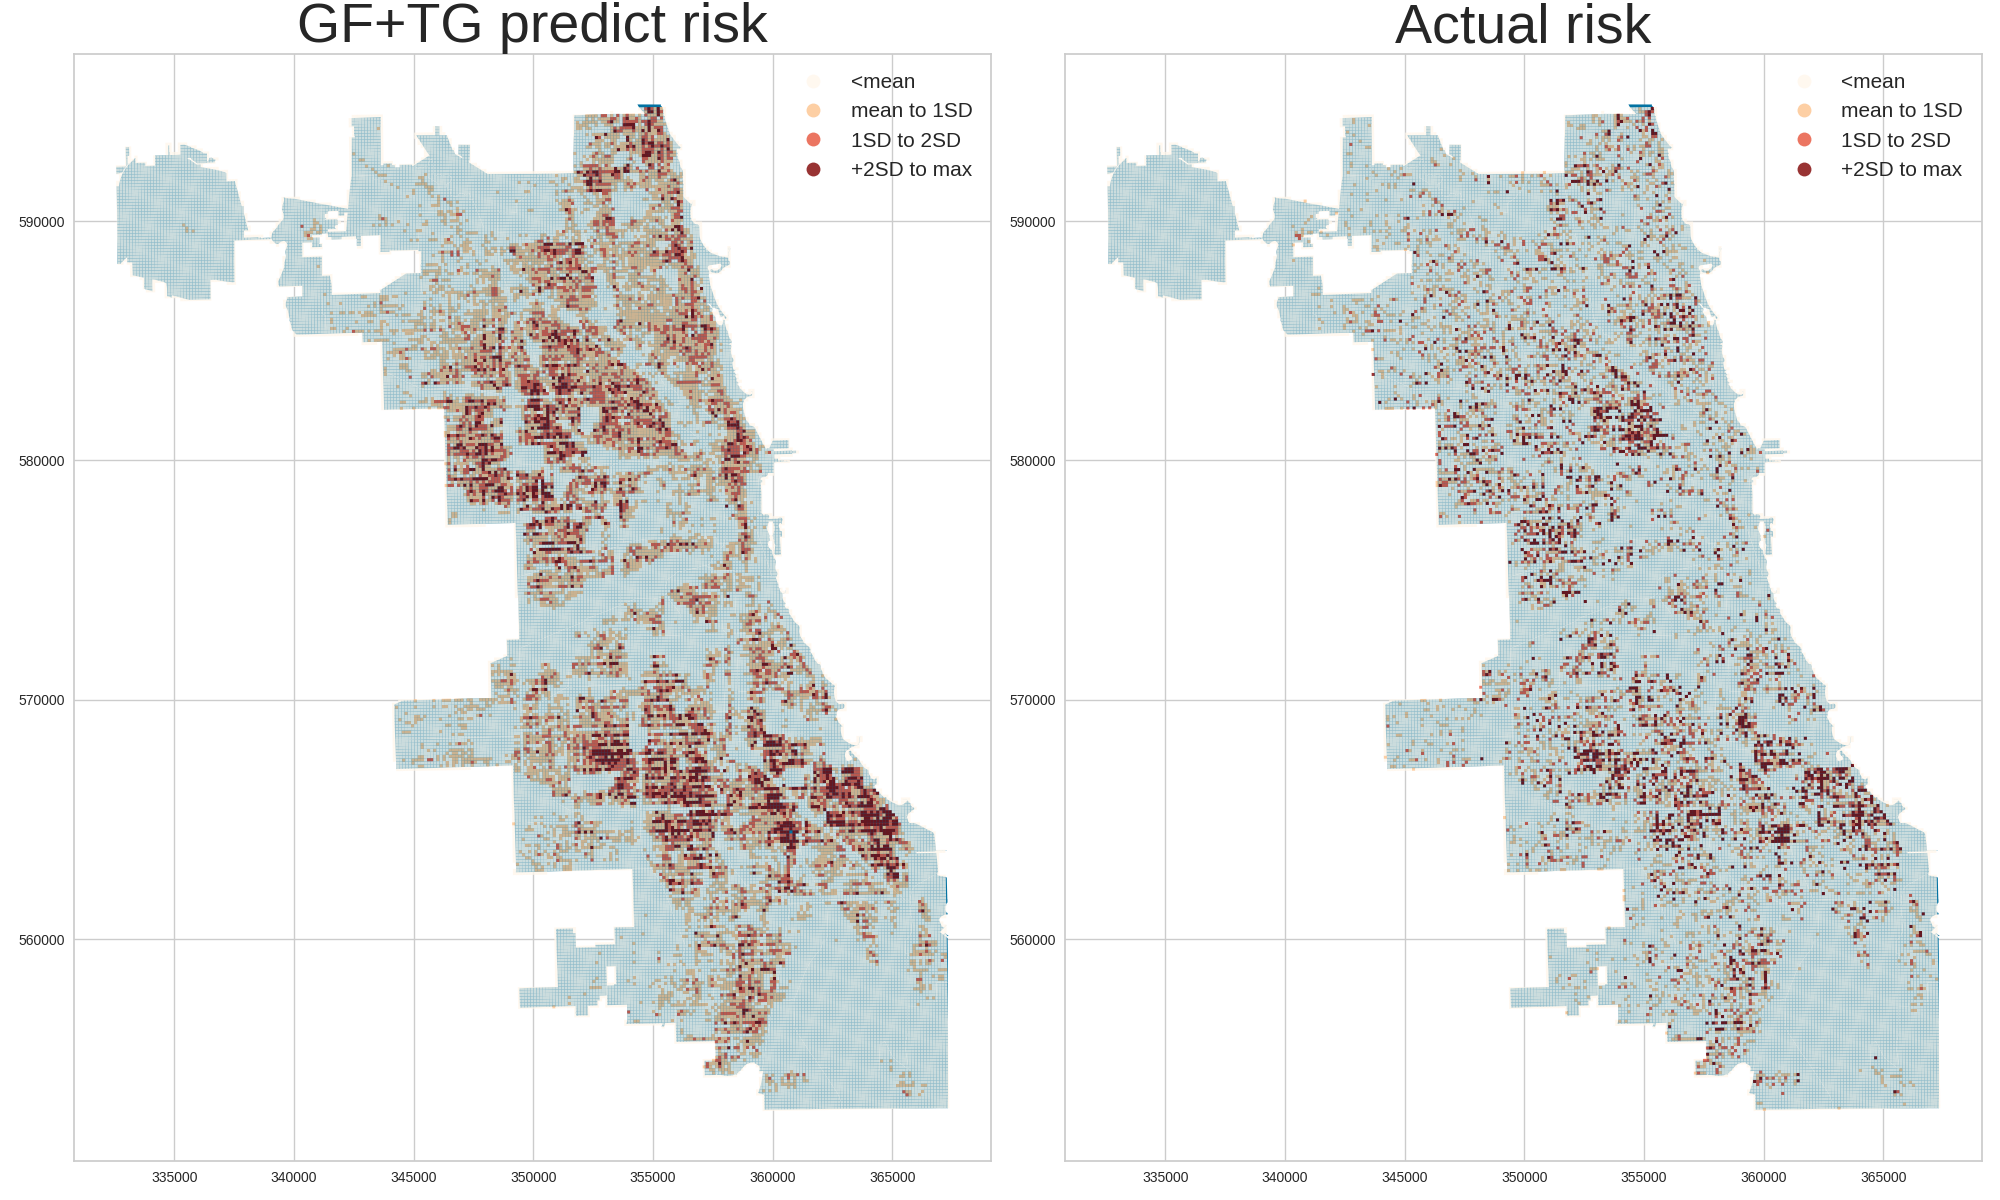
\includegraphics[scale=0.25]{./add-crime-timeseries-fig/GF+TG_riskmap.png}
  \caption{左:FG+TGによるリスクマップ 右:実際のリスクマップ}
  \label{fig:add-crime-timeseries-gf-tg-risk}
\end{figure}
%------------------------------------------
% confusion matrix
%------------------------------------------
\begin{figure}
  \centering % 図を中央寄せにする
  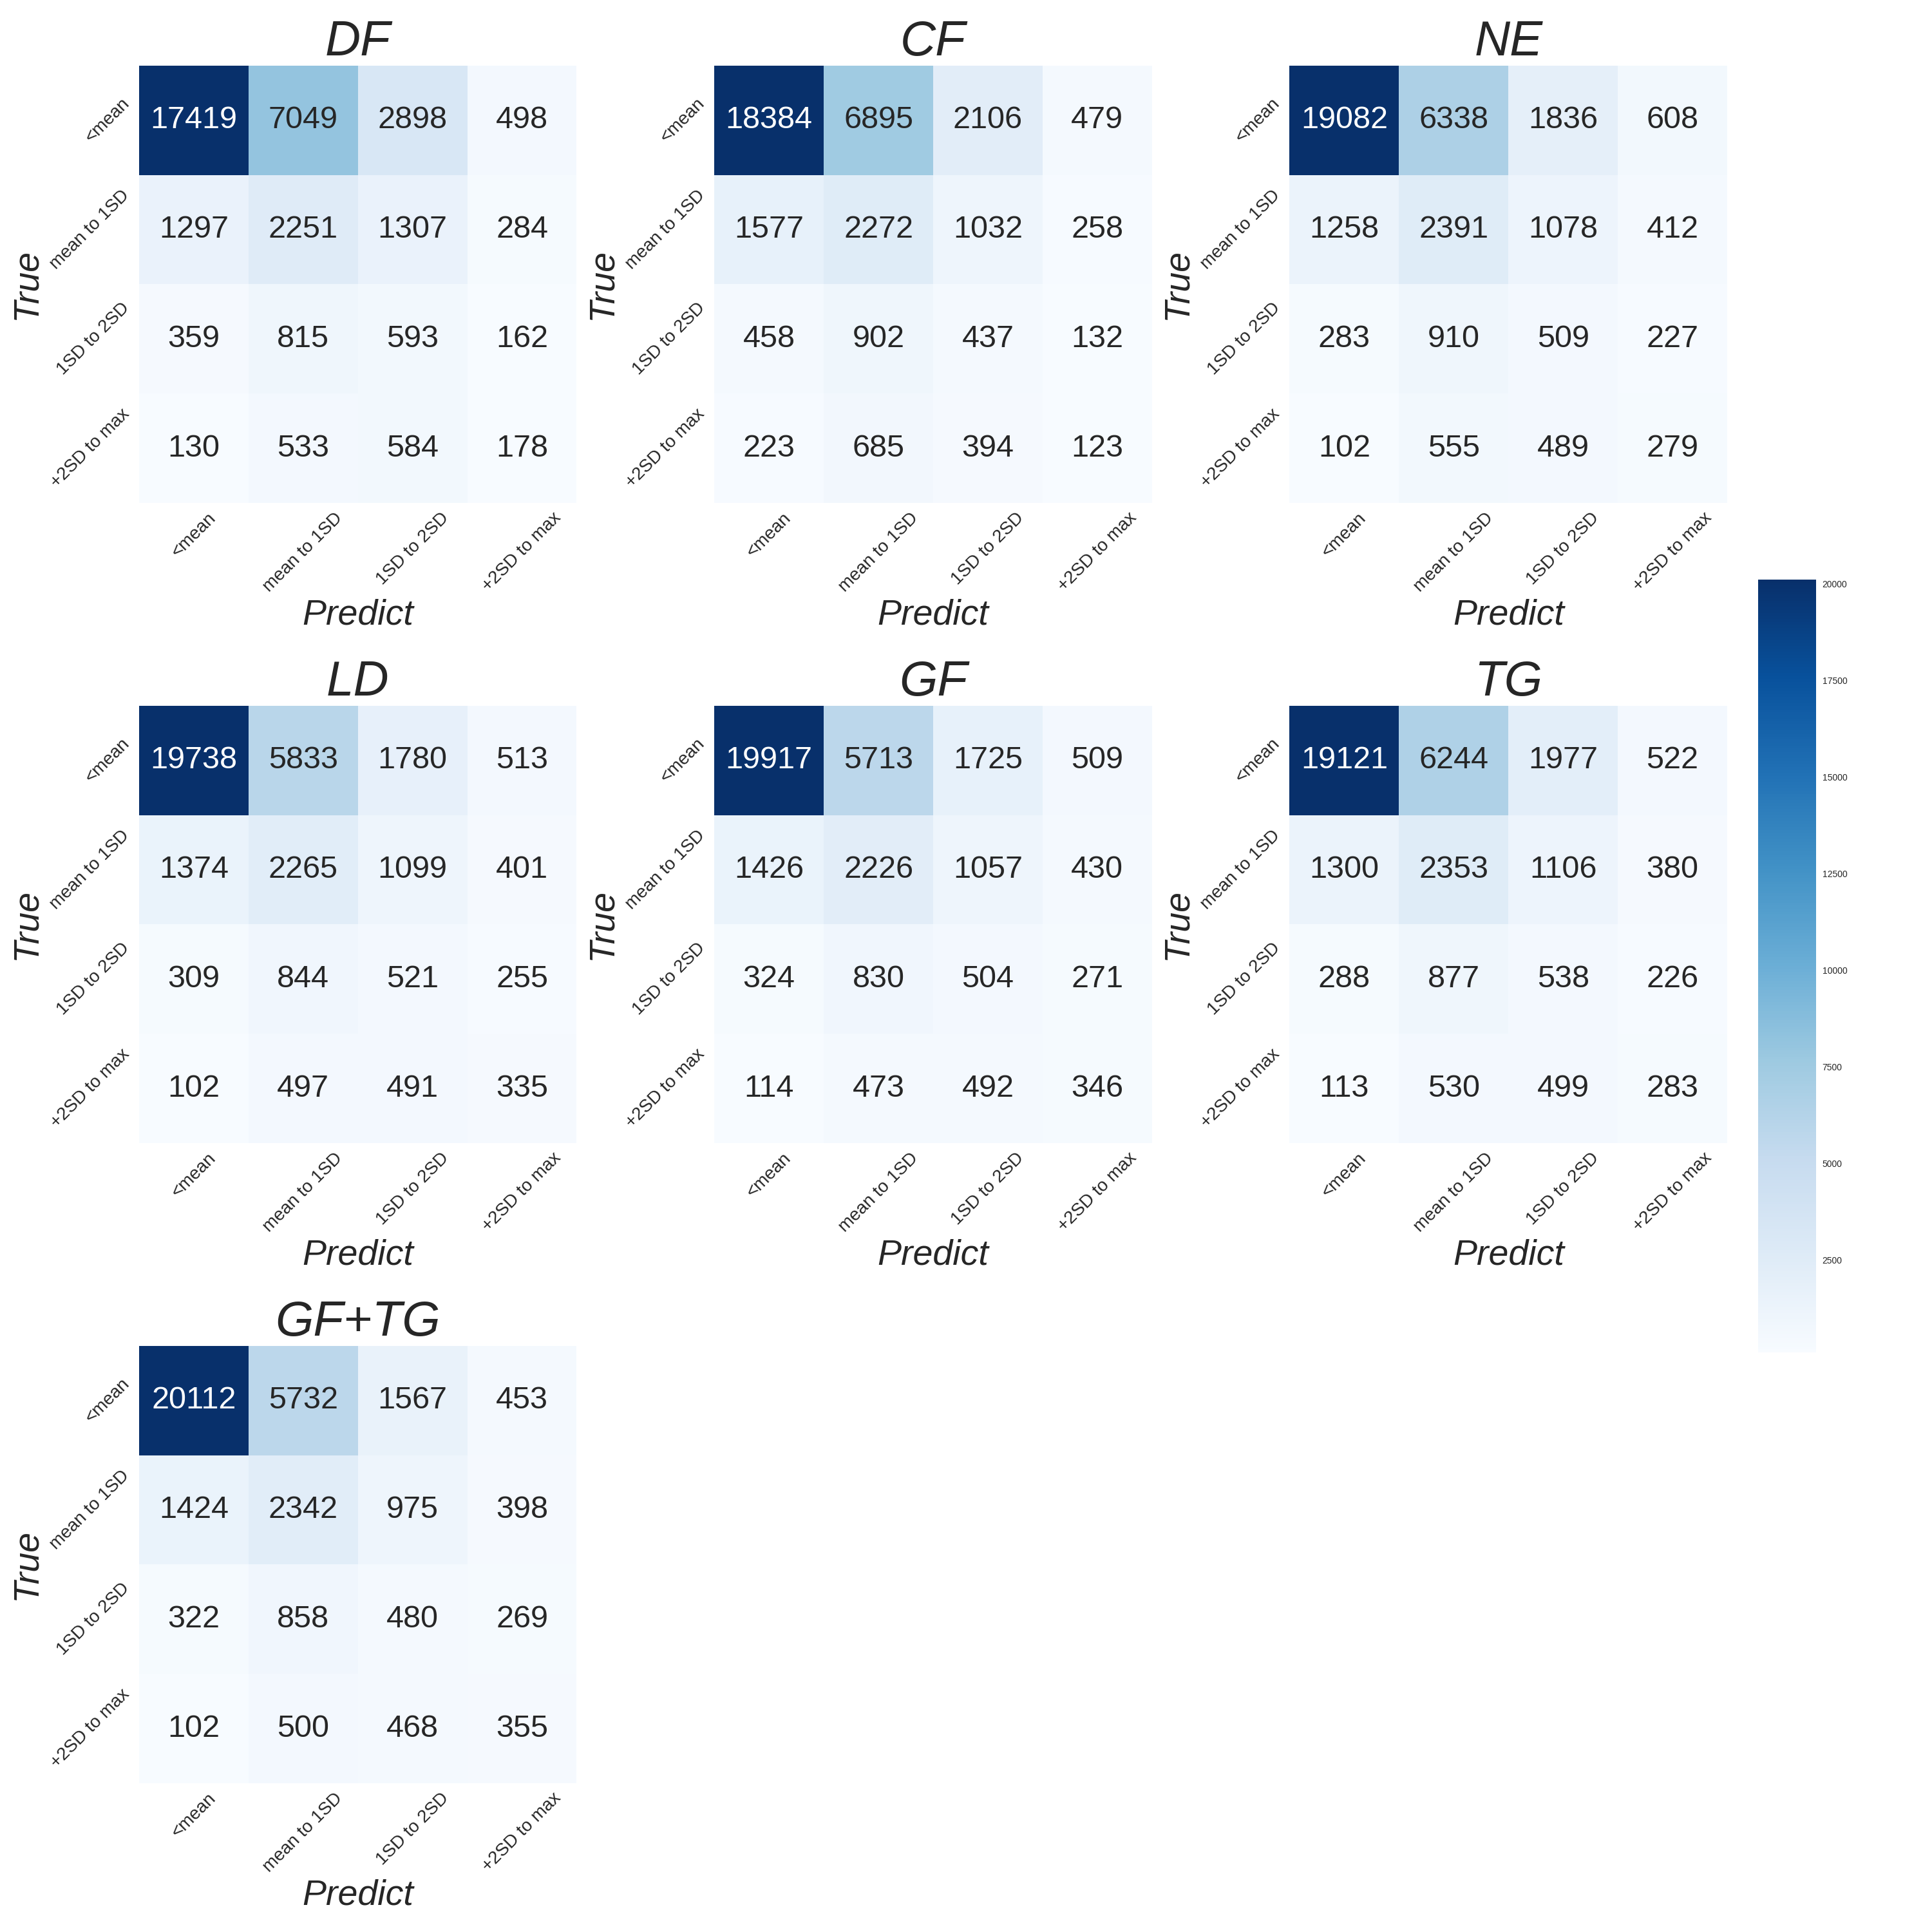
\includegraphics[scale=0.16]{./add-crime-timeseries-fig/crime_timeseries_four_cm.png}
  \caption{4カテゴリーの混同行列}
  \label{fig:add-crime-timeseries-4cm}
\end{figure}

\begin{figure}
  \centering % 図を中央寄せにする
  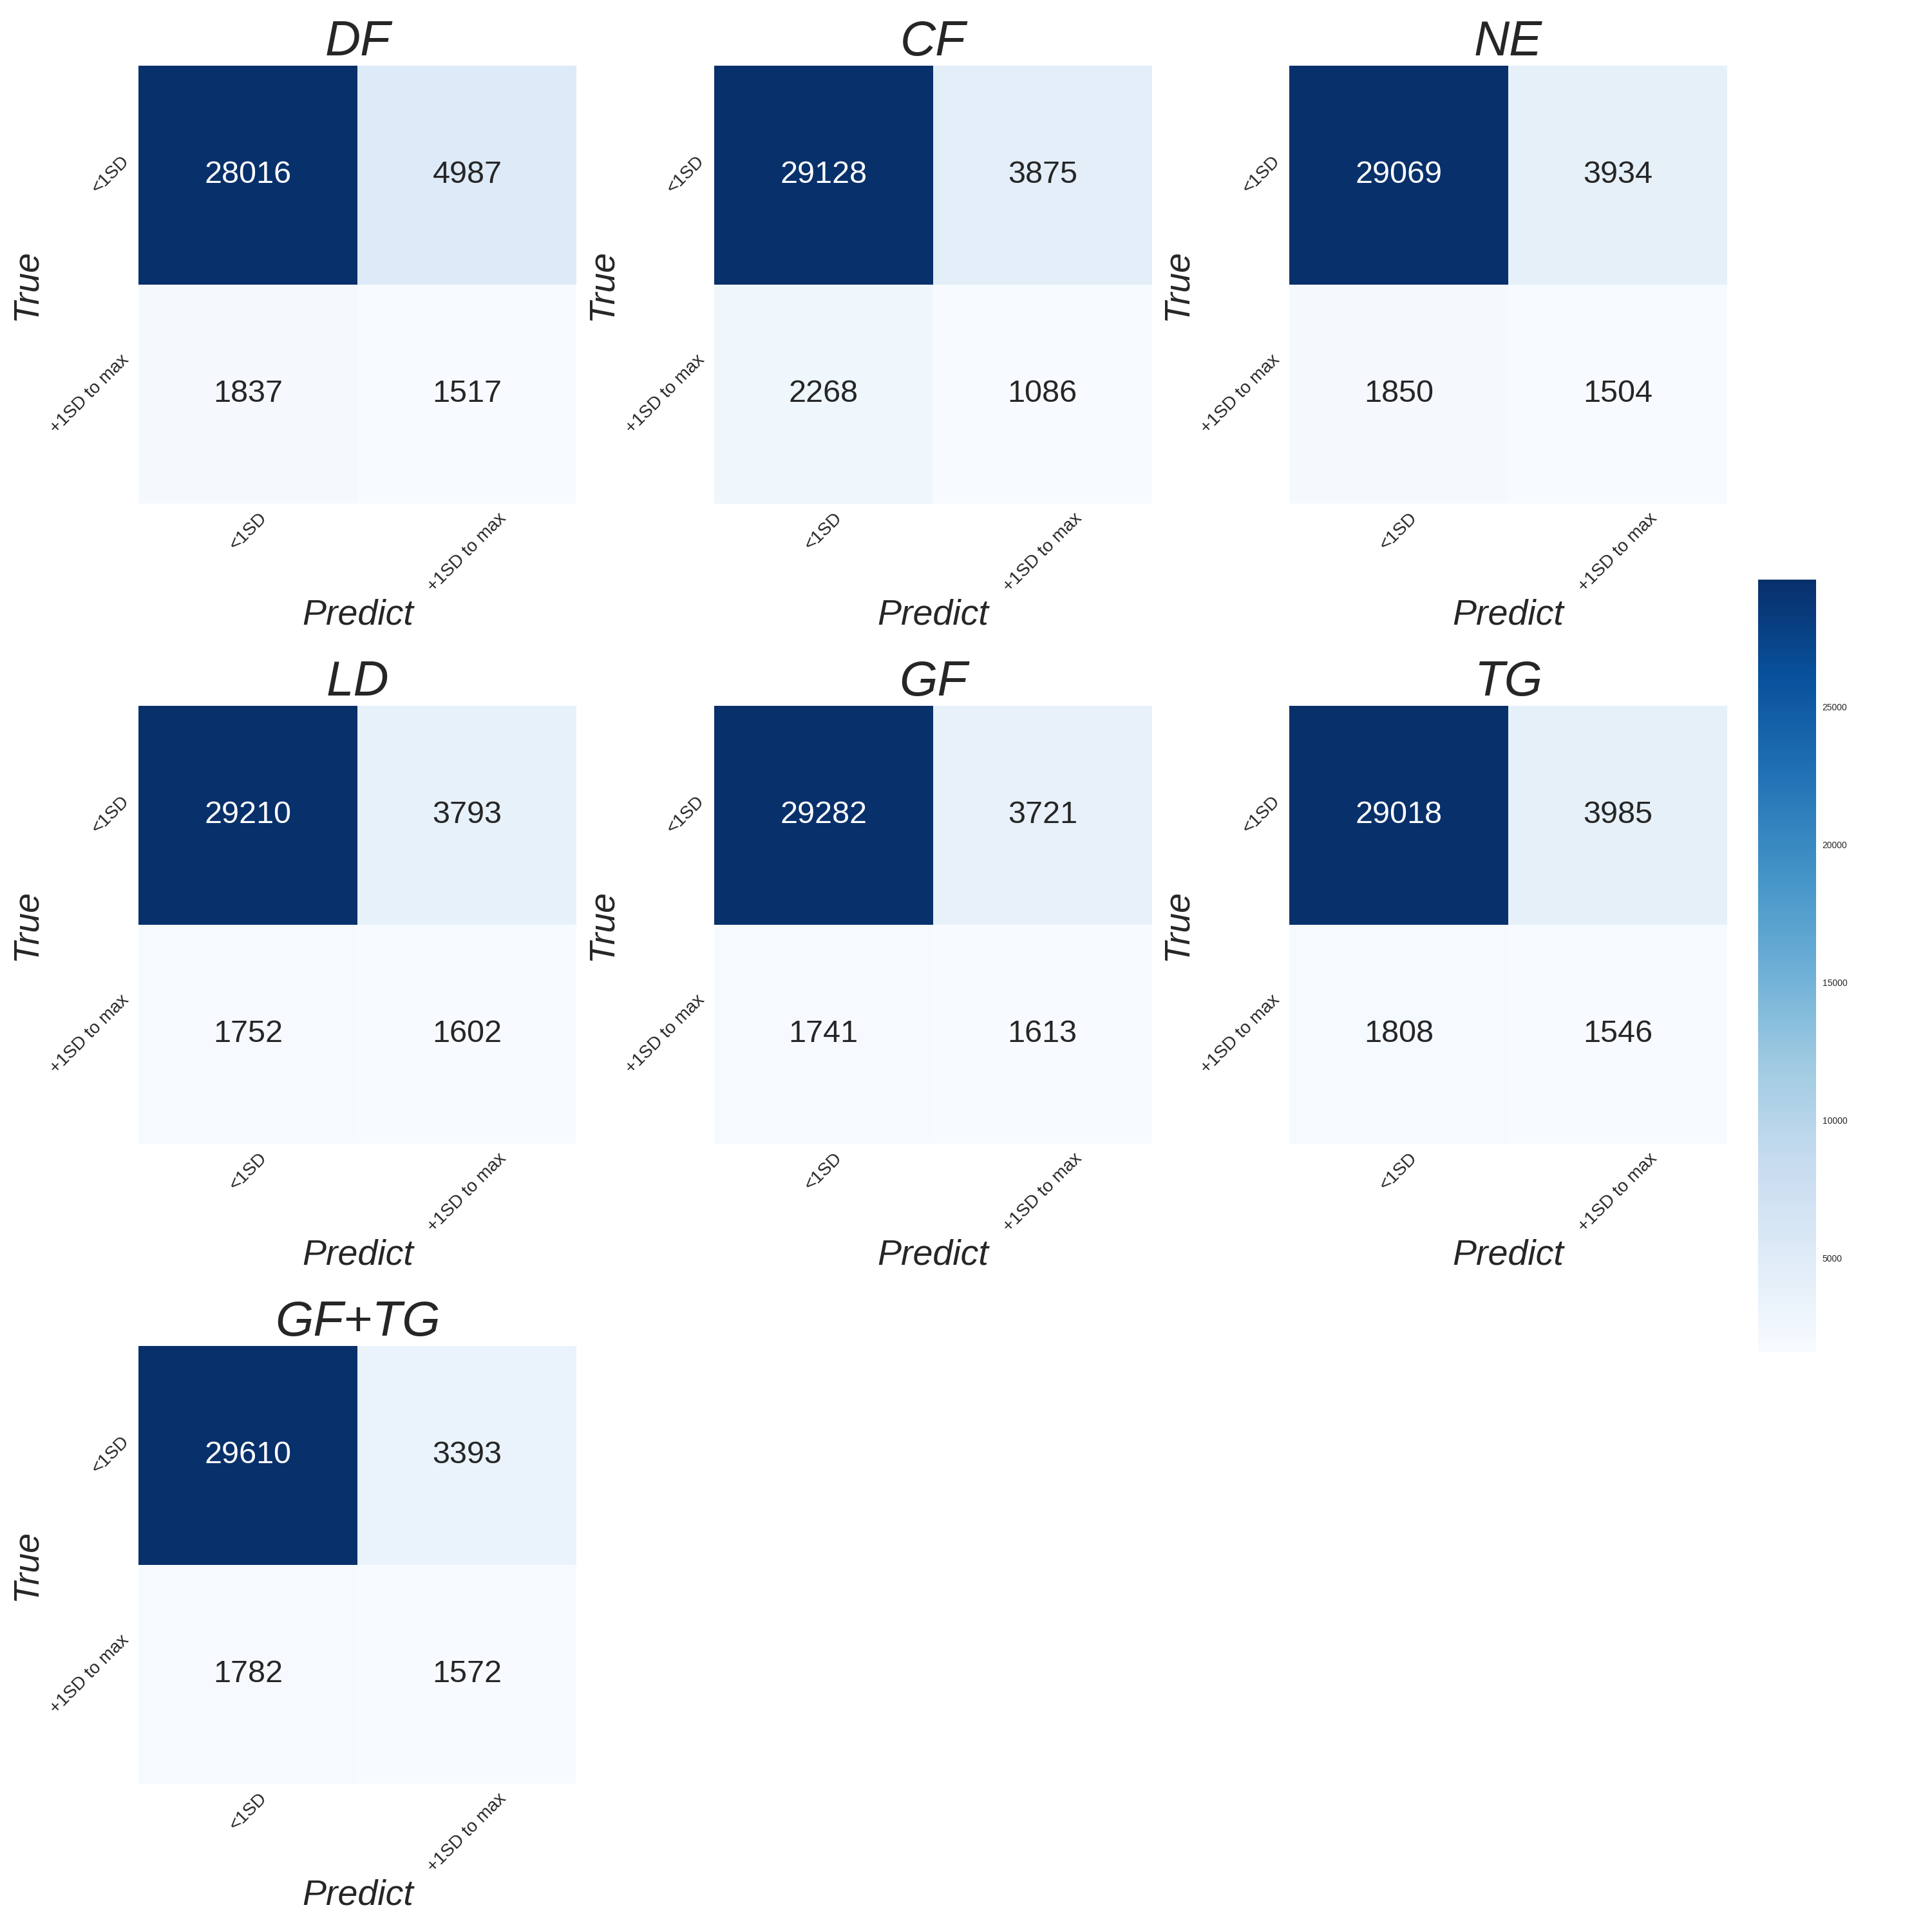
\includegraphics[scale=0.16]{./add-crime-timeseries-fig/crime_timeseries_two_cm.png}
  \caption{2カテゴリーの混同行列}
  \label{fig:add-crime-timeseries-2cm}
\end{figure}
% ---------------------------------
% FNFPplot
% ---------------------------------
\begin{figure}
  \centering % 図を中央寄せにする
  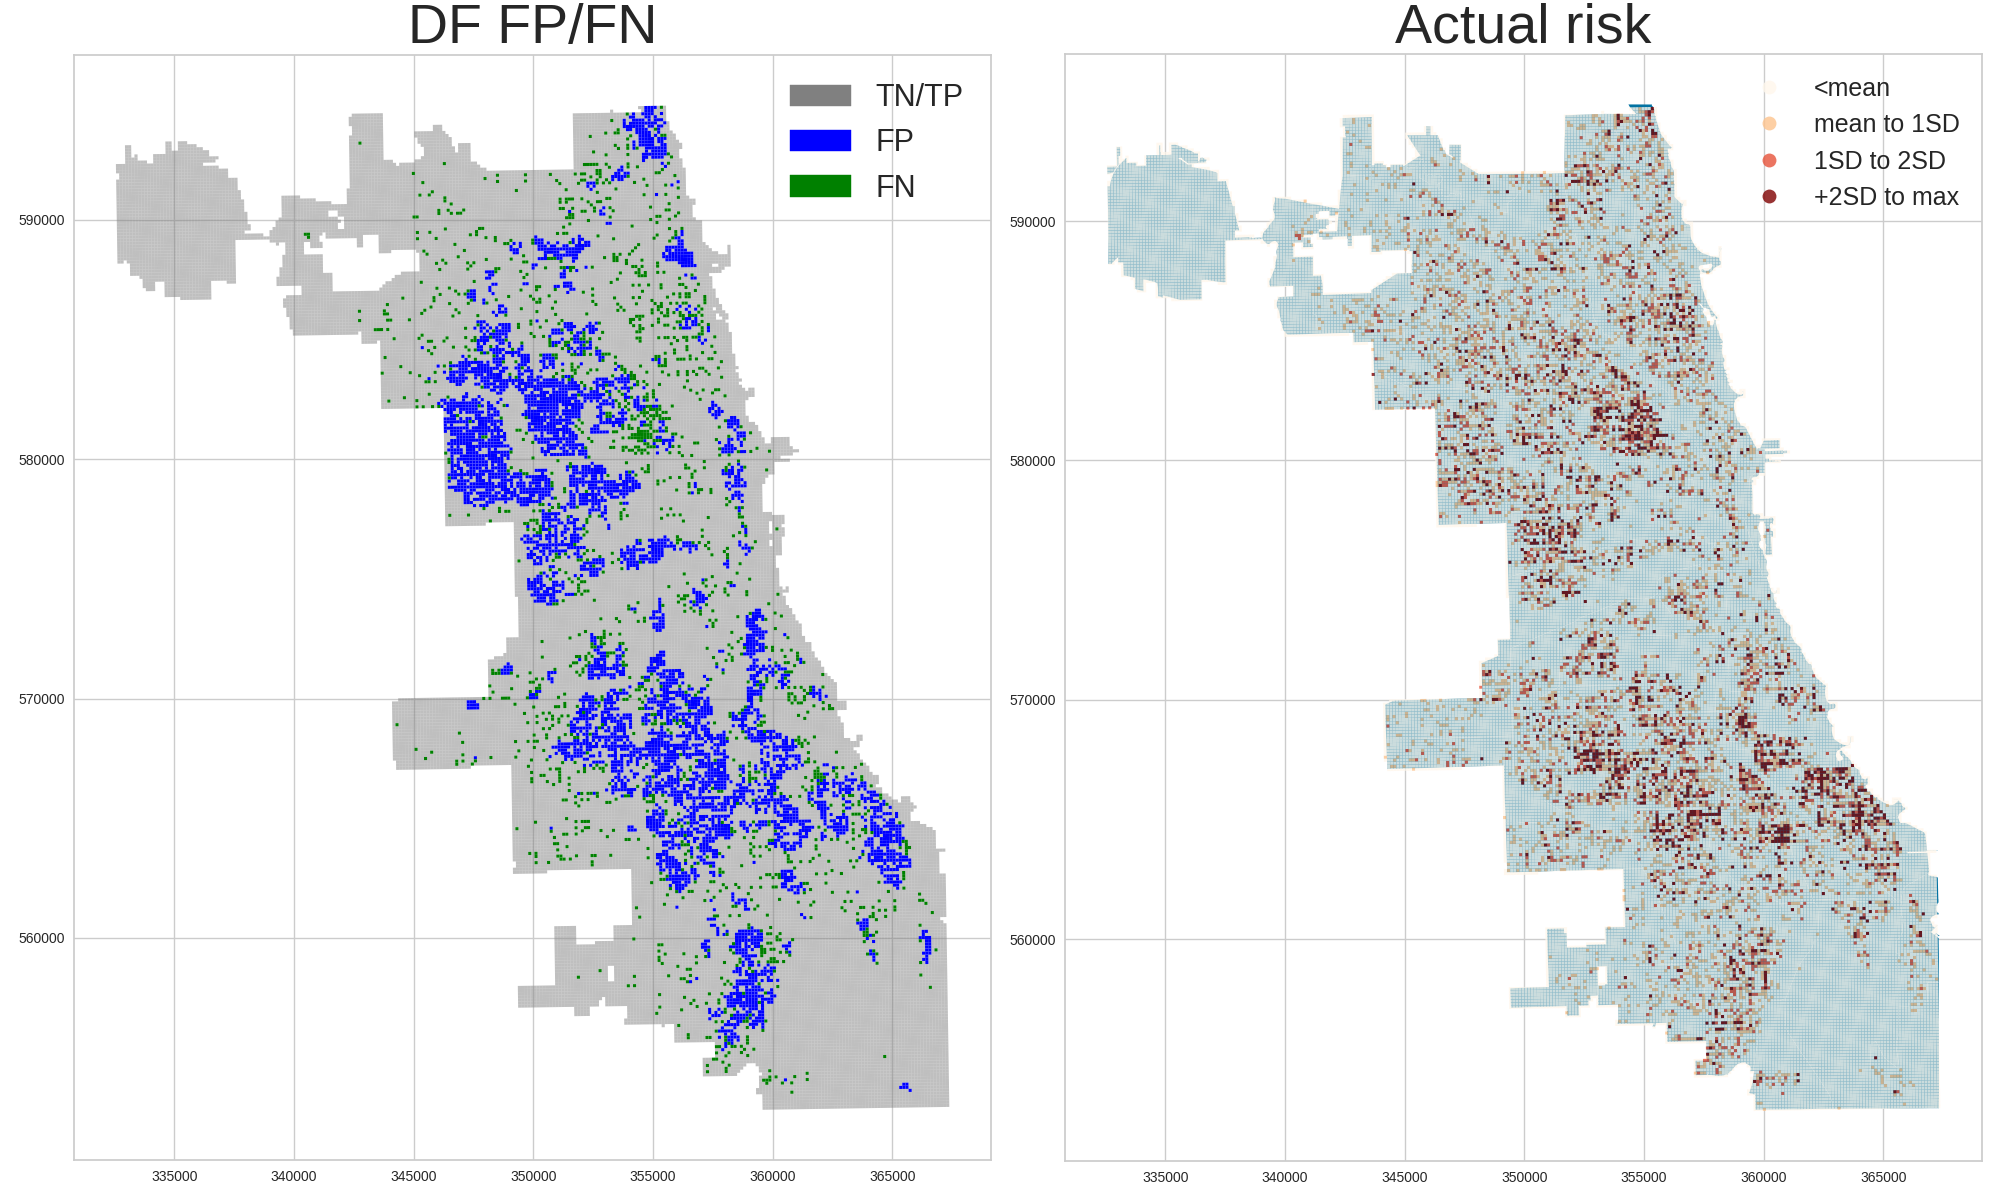
\includegraphics[scale=0.25]{./add-crime-timeseries-fig/DF_fnp.png}
  \caption{左:DFのFPFN 右:実際のリスクマップ}
  \label{fig:add-crime-timeseries-df-fnp}
\end{figure}

\begin{figure}
  \centering % 図を中央寄せにする
  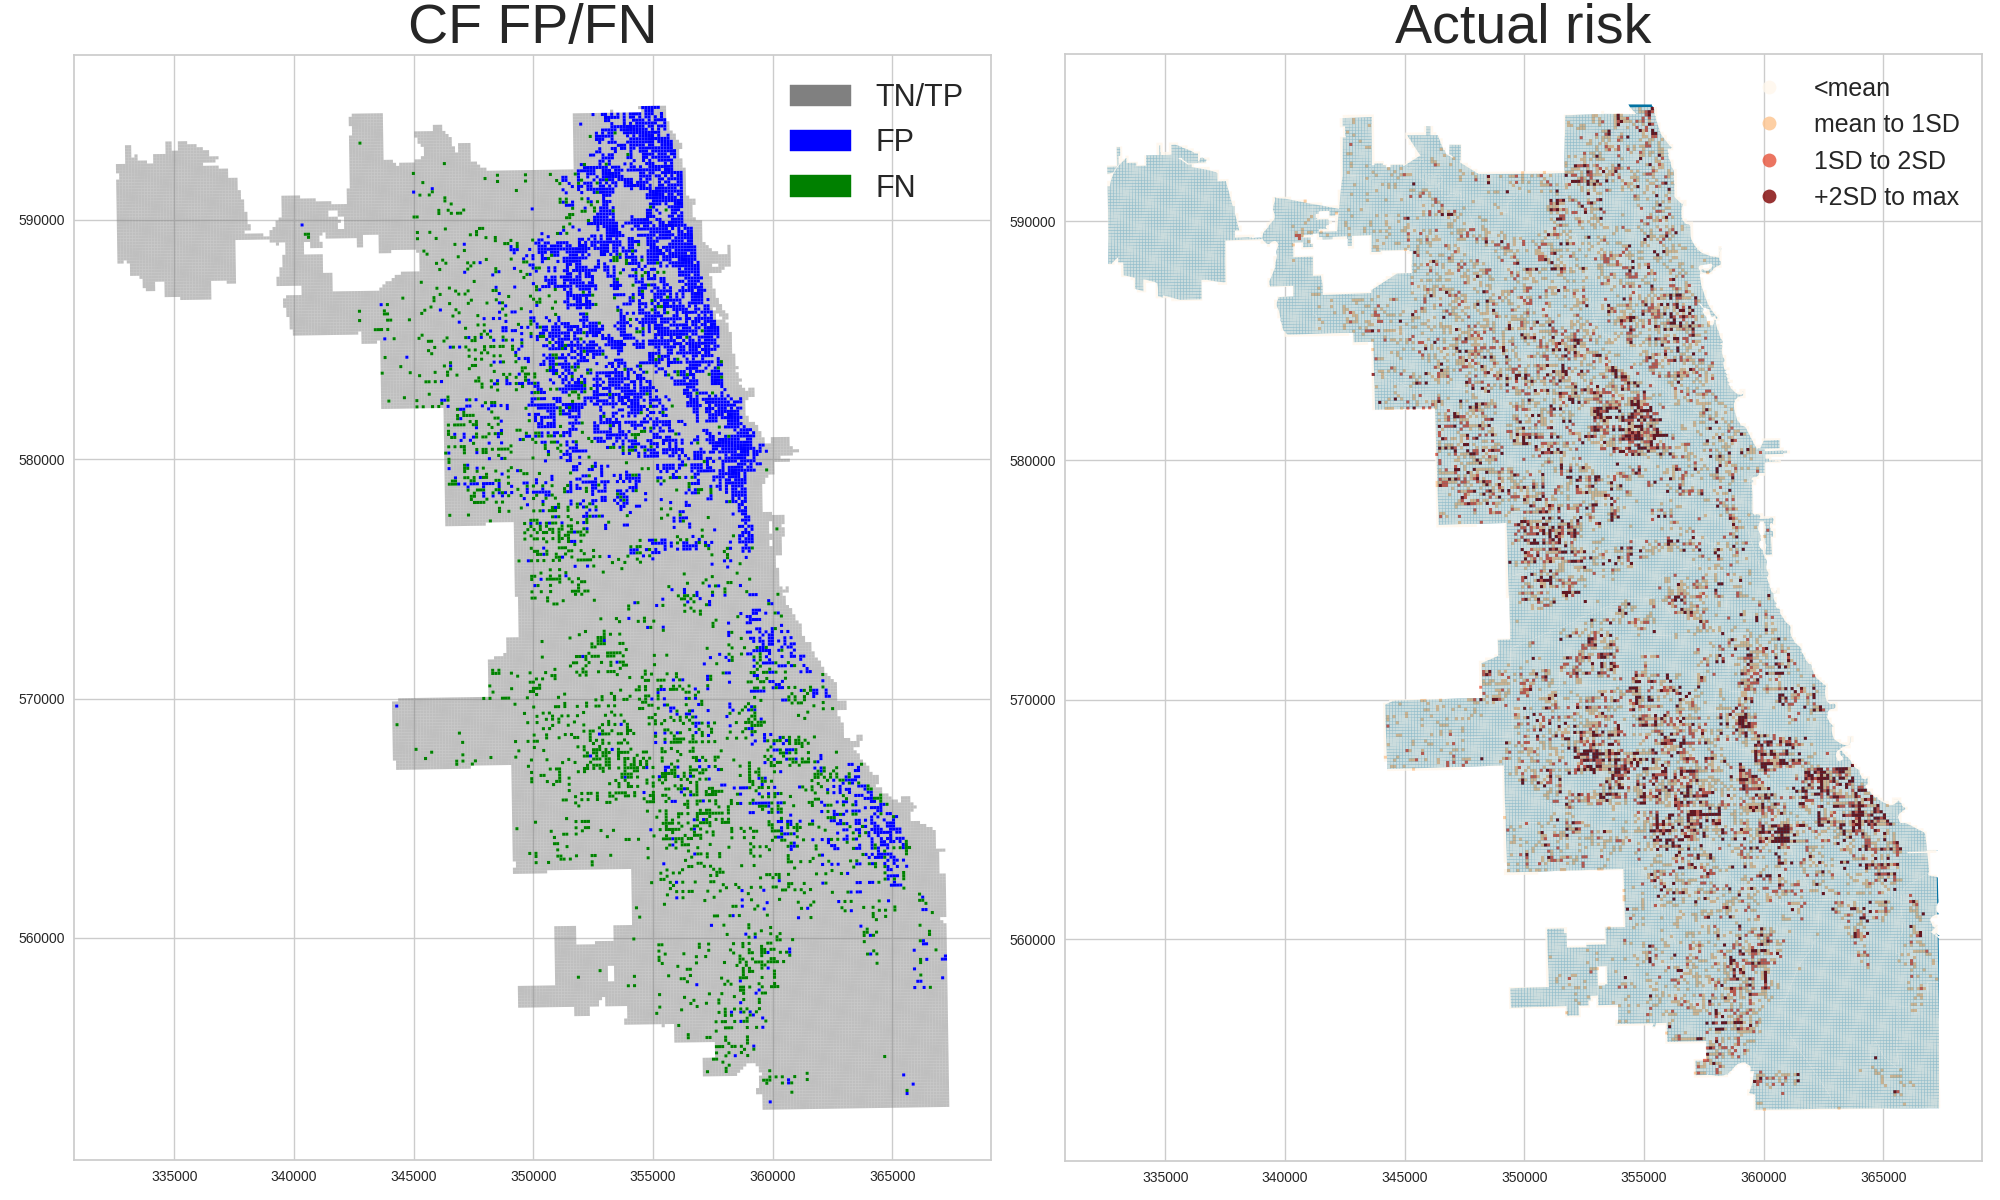
\includegraphics[scale=0.25]{./add-crime-timeseries-fig/CF_fnp.png}
  \caption{左:CFのFPFN 右:実際のリスクマップ}
  \label{fig:add-crime-timeseries-cf-fnp}
\end{figure}

\begin{figure}
  \centering % 図を中央寄せにする
  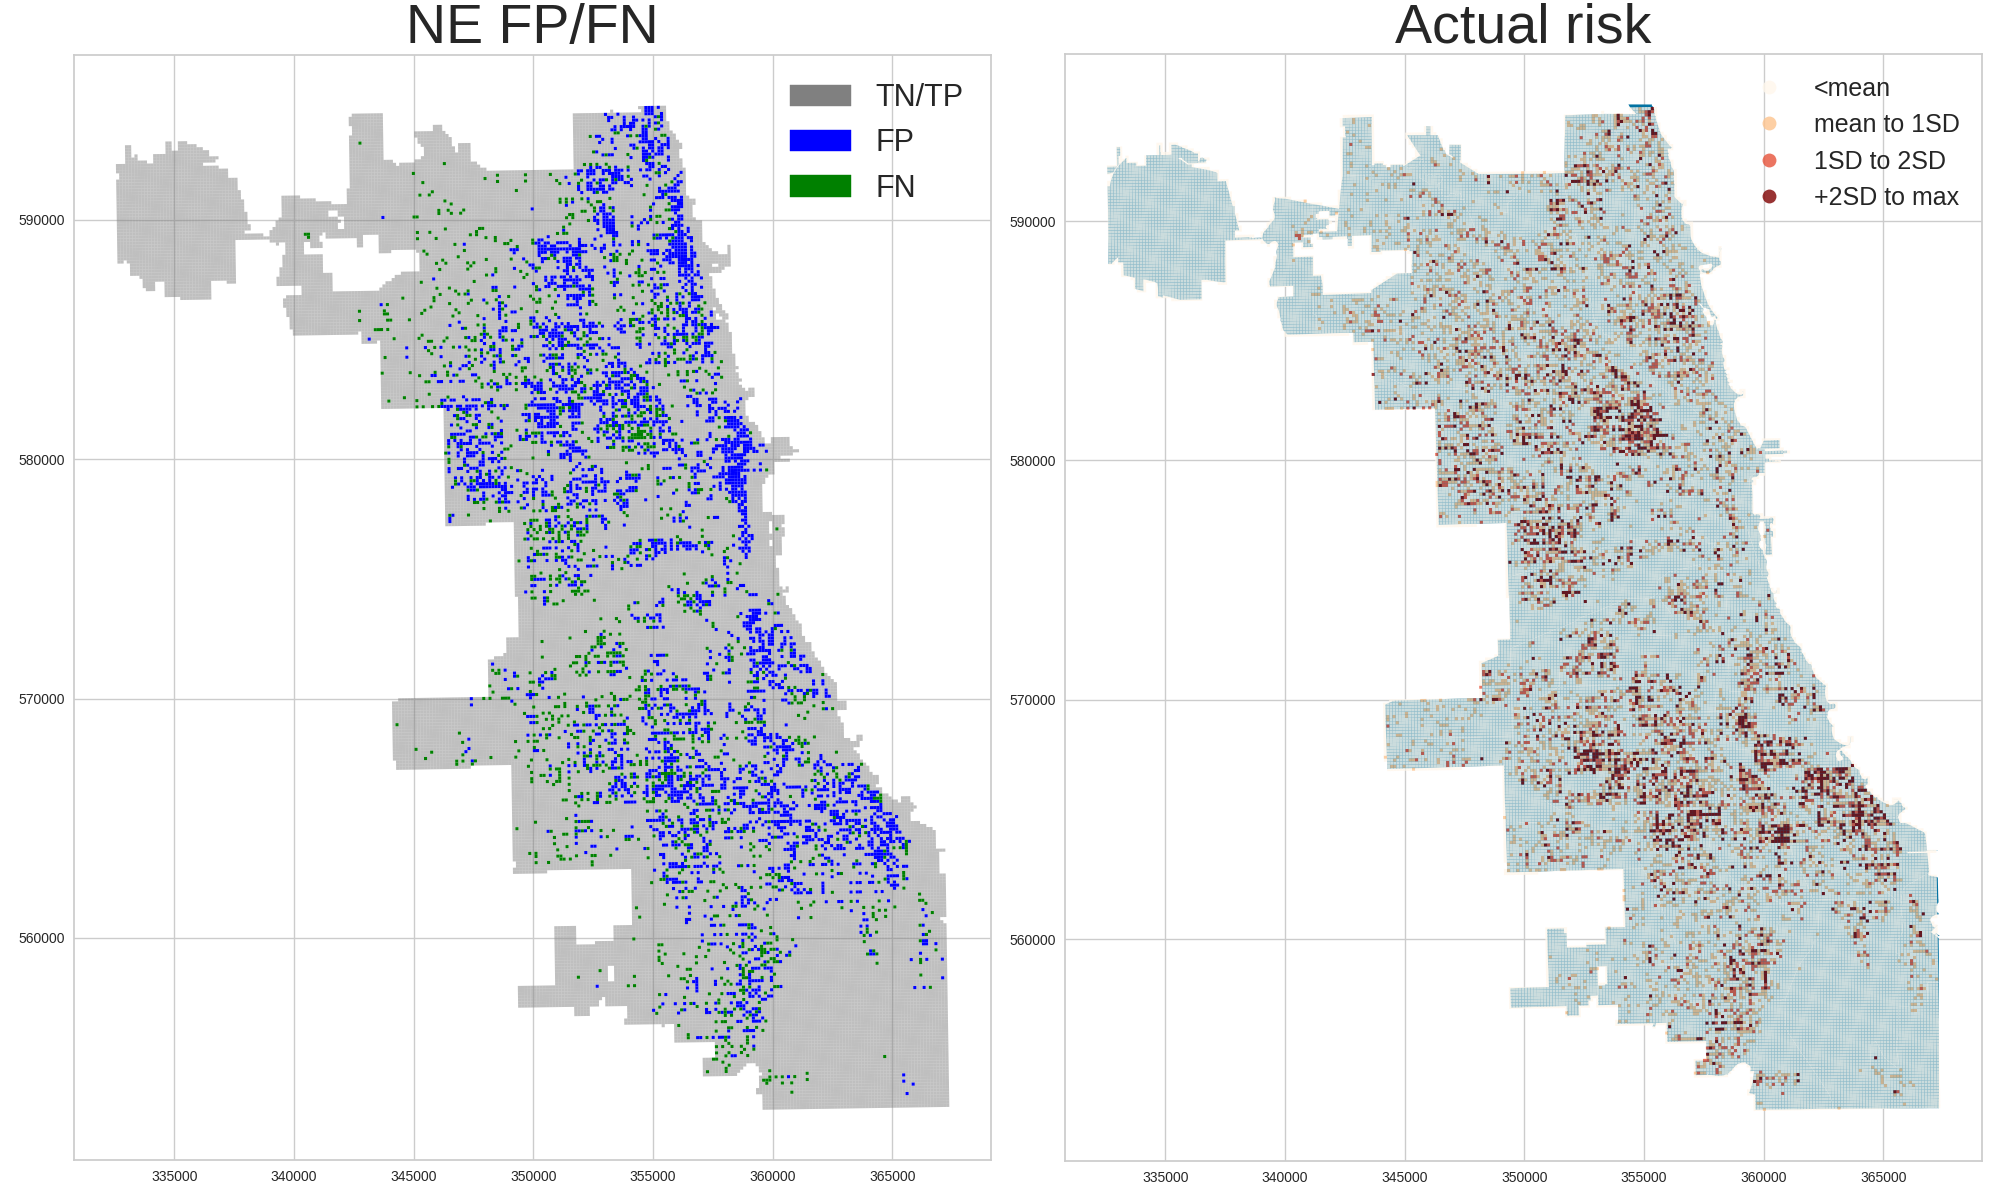
\includegraphics[scale=0.25]{./add-crime-timeseries-fig/NE_fnp.png}
  \caption{左:NEのFPFN 右:実際のリスクマップ}
  \label{fig:add-crime-timeseries-ne-fnp}
\end{figure}

\begin{figure}
  \centering % 図を中央寄せにする
  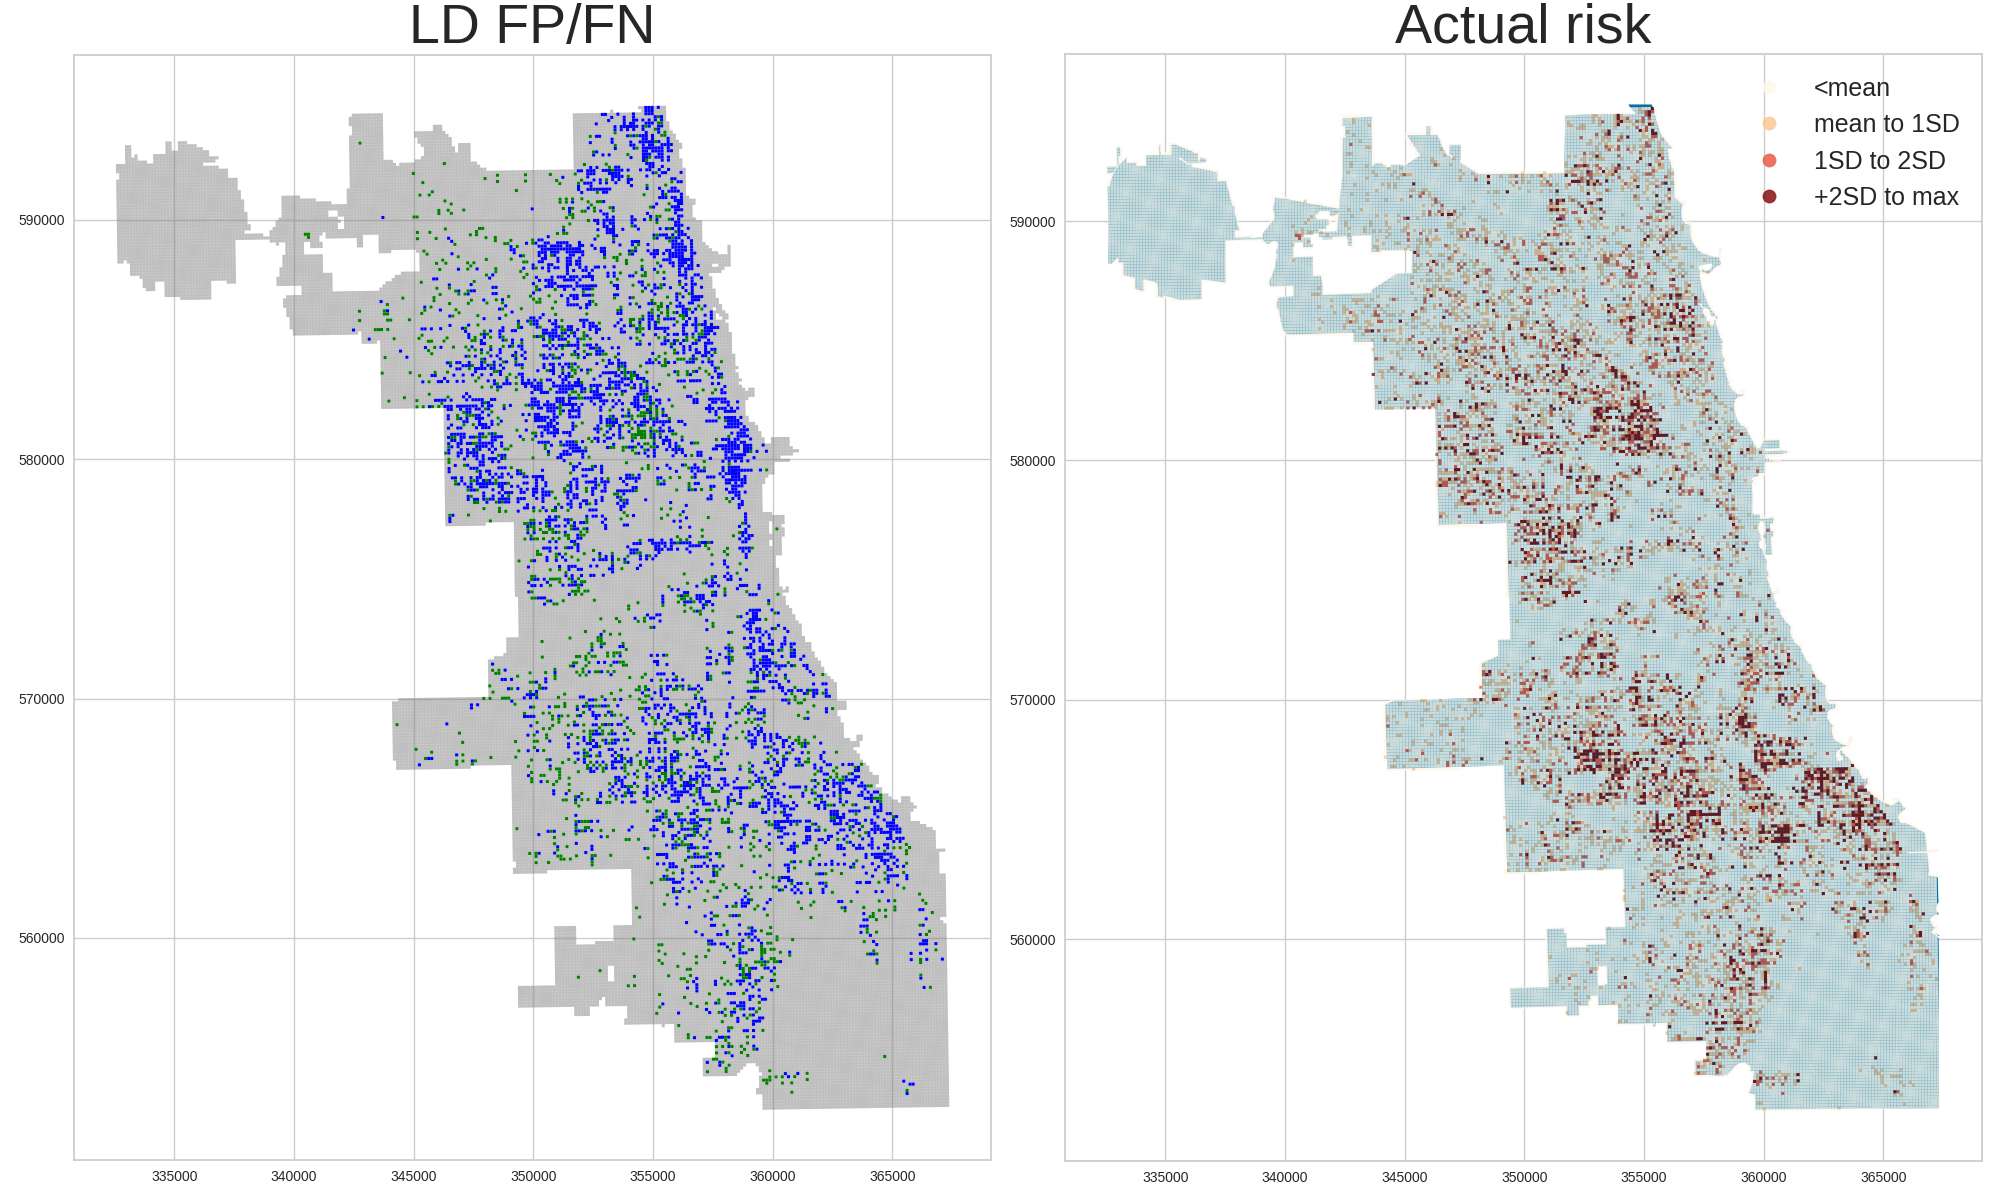
\includegraphics[scale=0.25]{./add-crime-timeseries-fig/LD_fnp.png}
  \caption{左:LDのFPFN 右:実際のリスクマップ}
  \label{fig:add-crime-timeseries-ld-fnp}
\end{figure}

\begin{figure}
  \centering % 図を中央寄せにする
  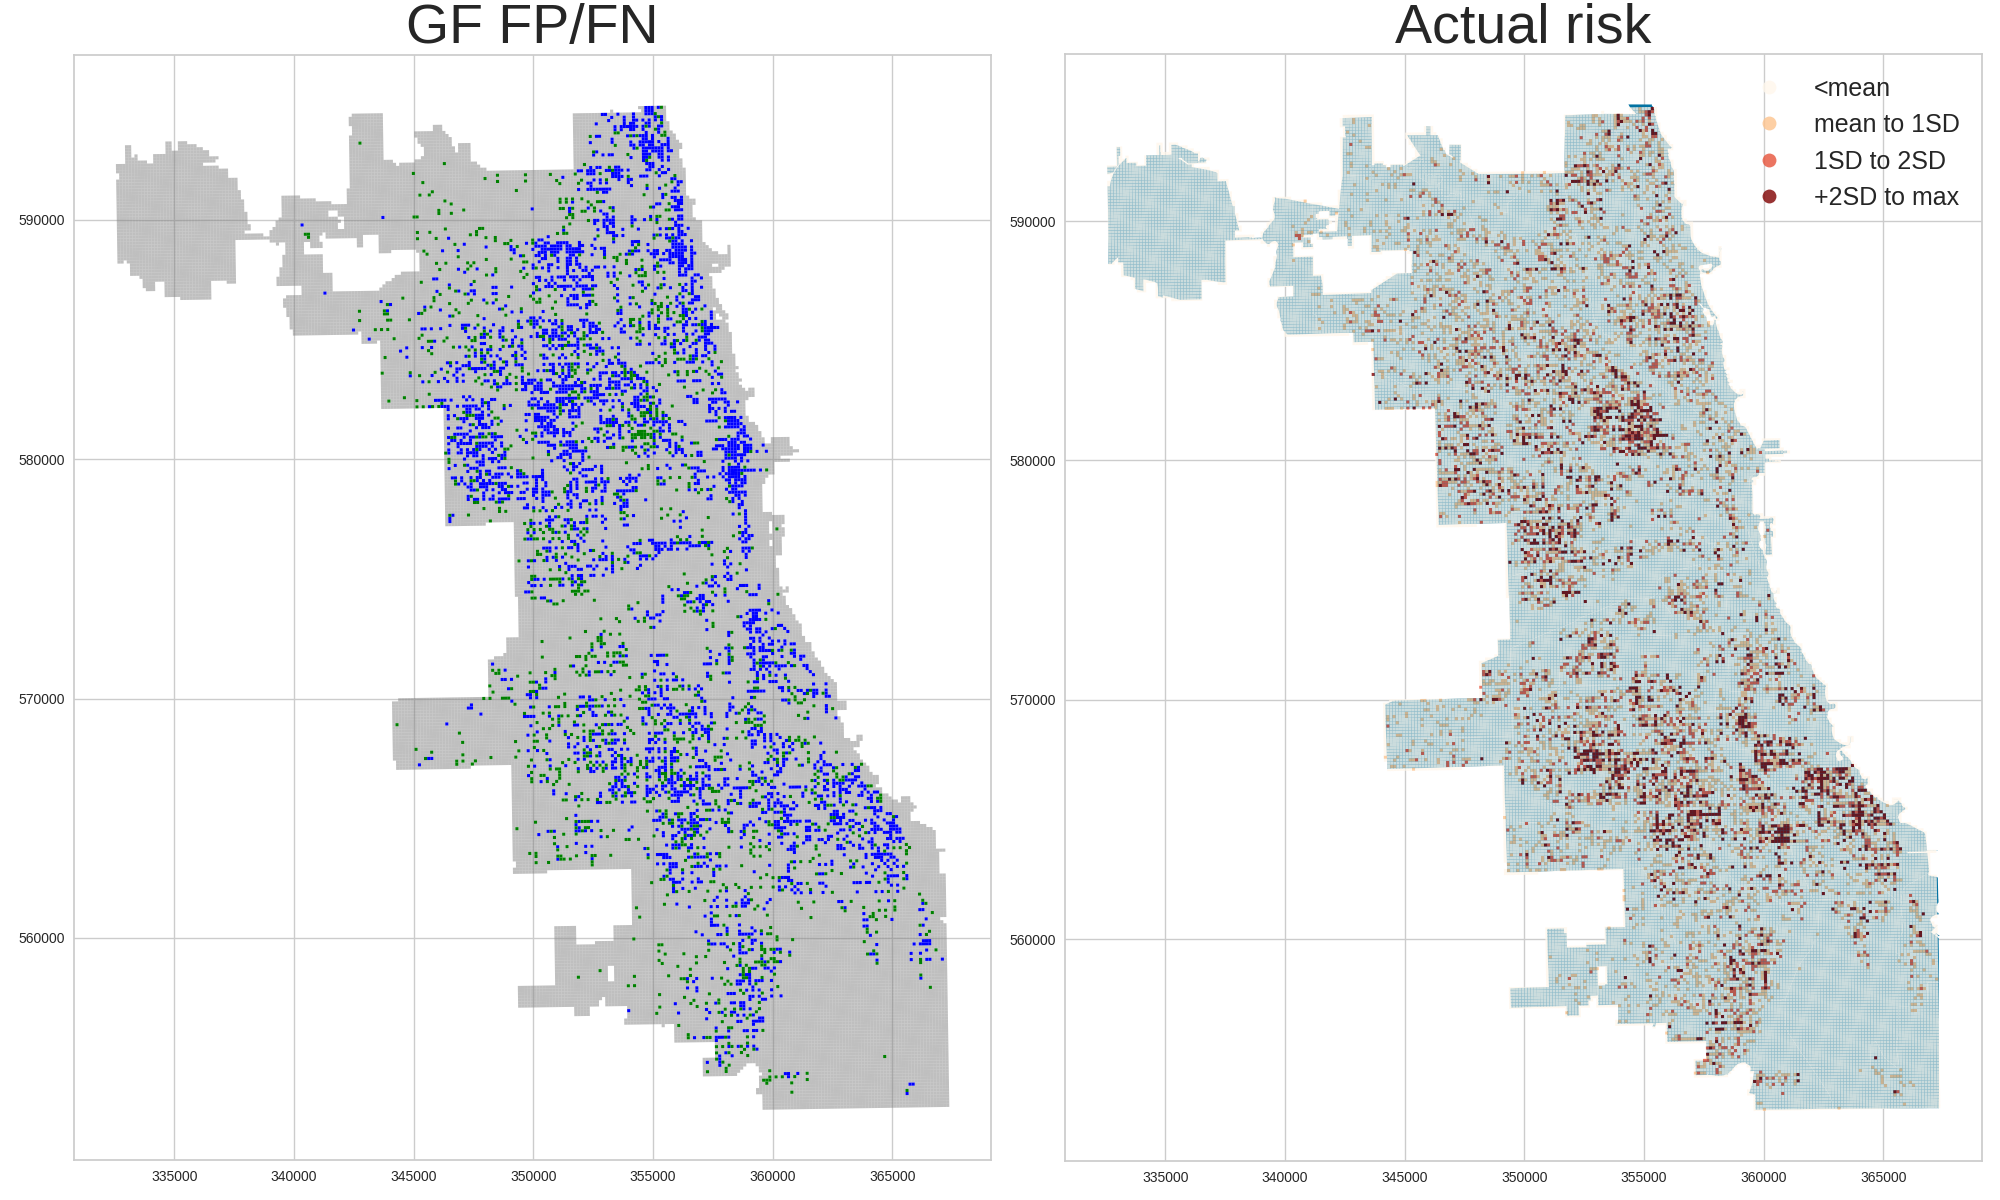
\includegraphics[scale=0.25]{./add-crime-timeseries-fig/GF_fnp.png}
  \caption{左:GFのFPFN 右:実際のリスクマップ}
  \label{fig:add-crime-timeseries-gf-fnp}
\end{figure}

\begin{figure}
  \centering % 図を中央寄せにする
  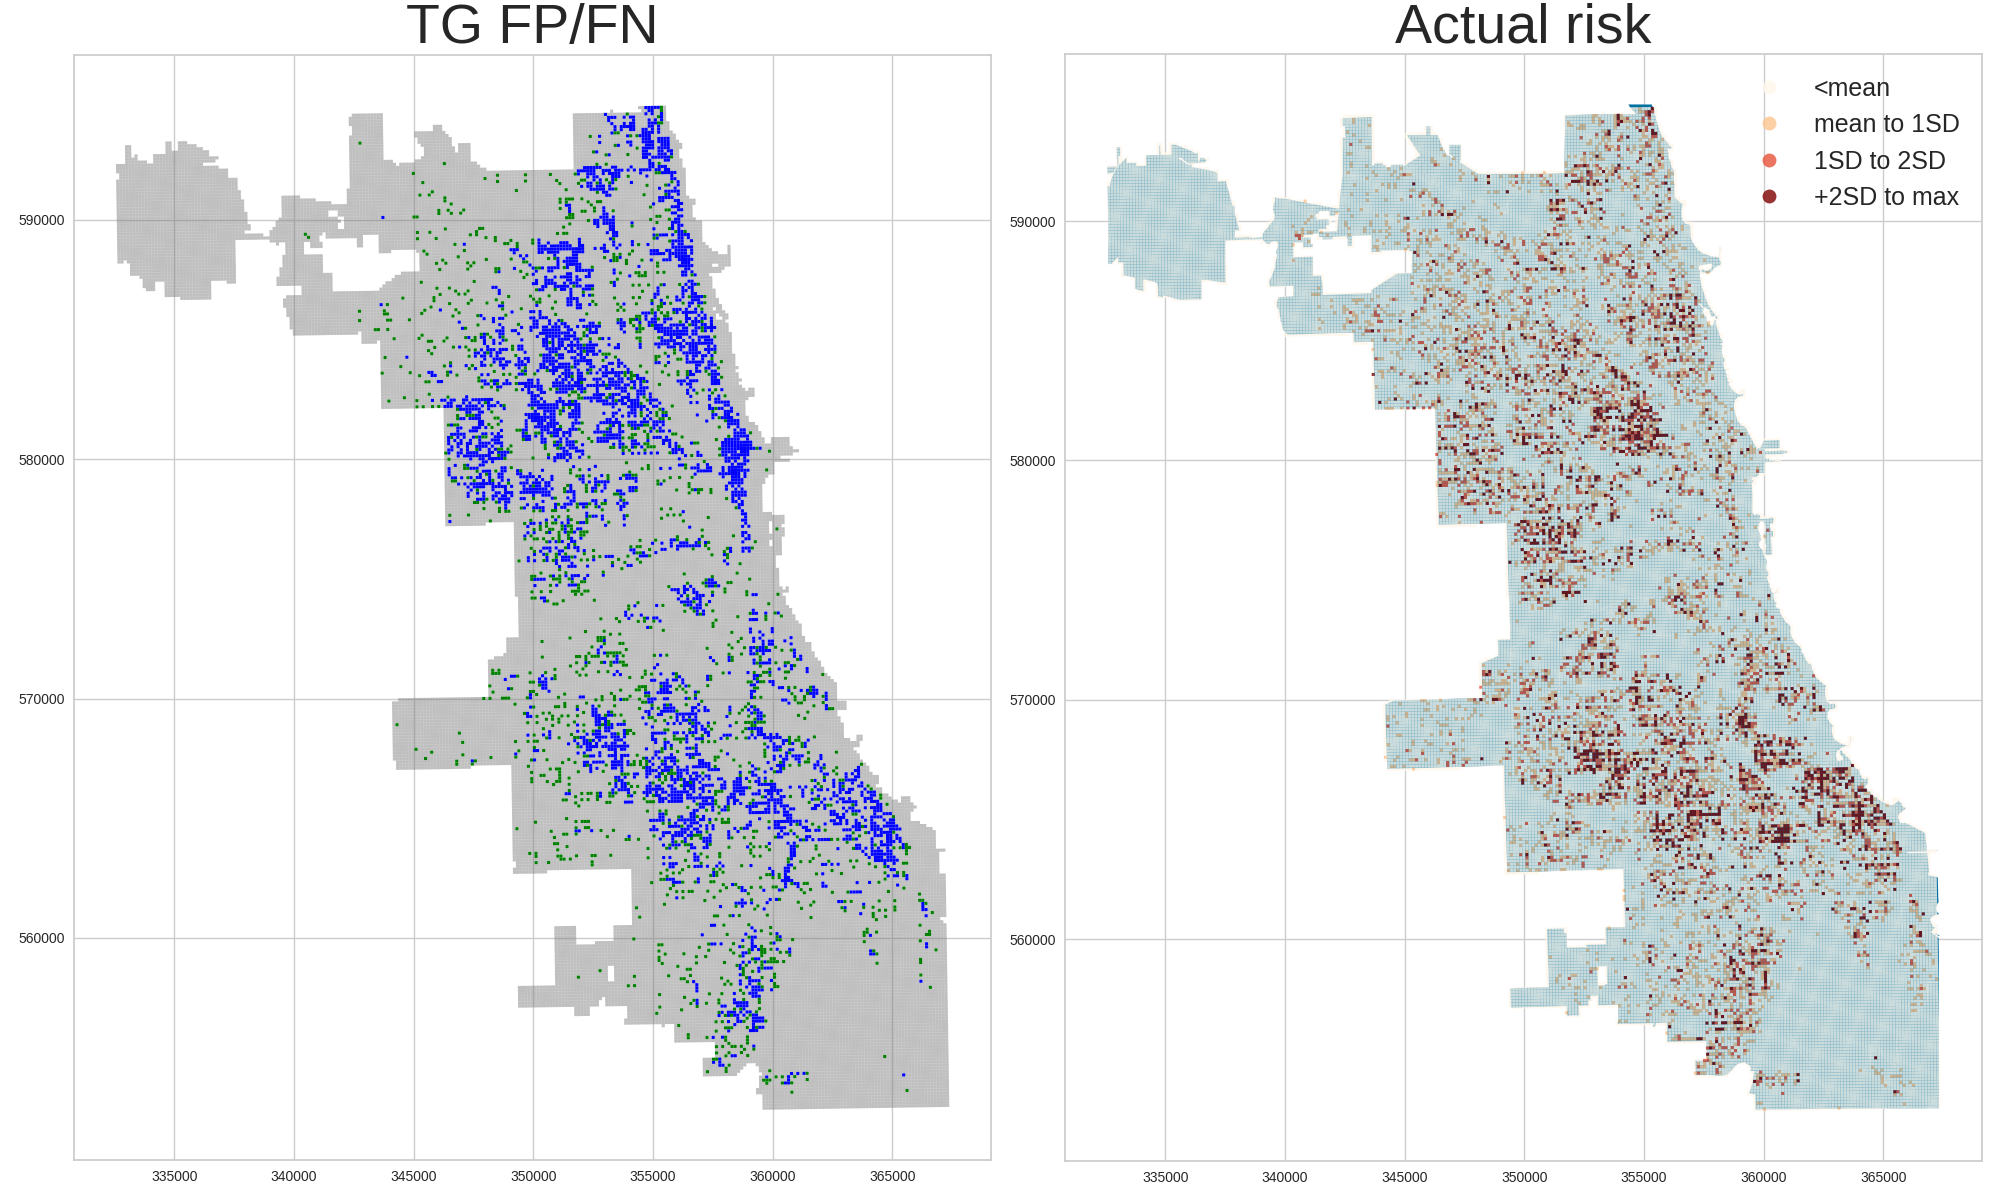
\includegraphics[scale=0.25]{./add-crime-timeseries-fig/TG_fnp.png}
  \caption{左:TGのFPFN 右:実際のリスクマップ}
  \label{fig:add-crime-timeseries-tg-fnp}
\end{figure}

\begin{figure}
  \centering % 図を中央寄せにする
  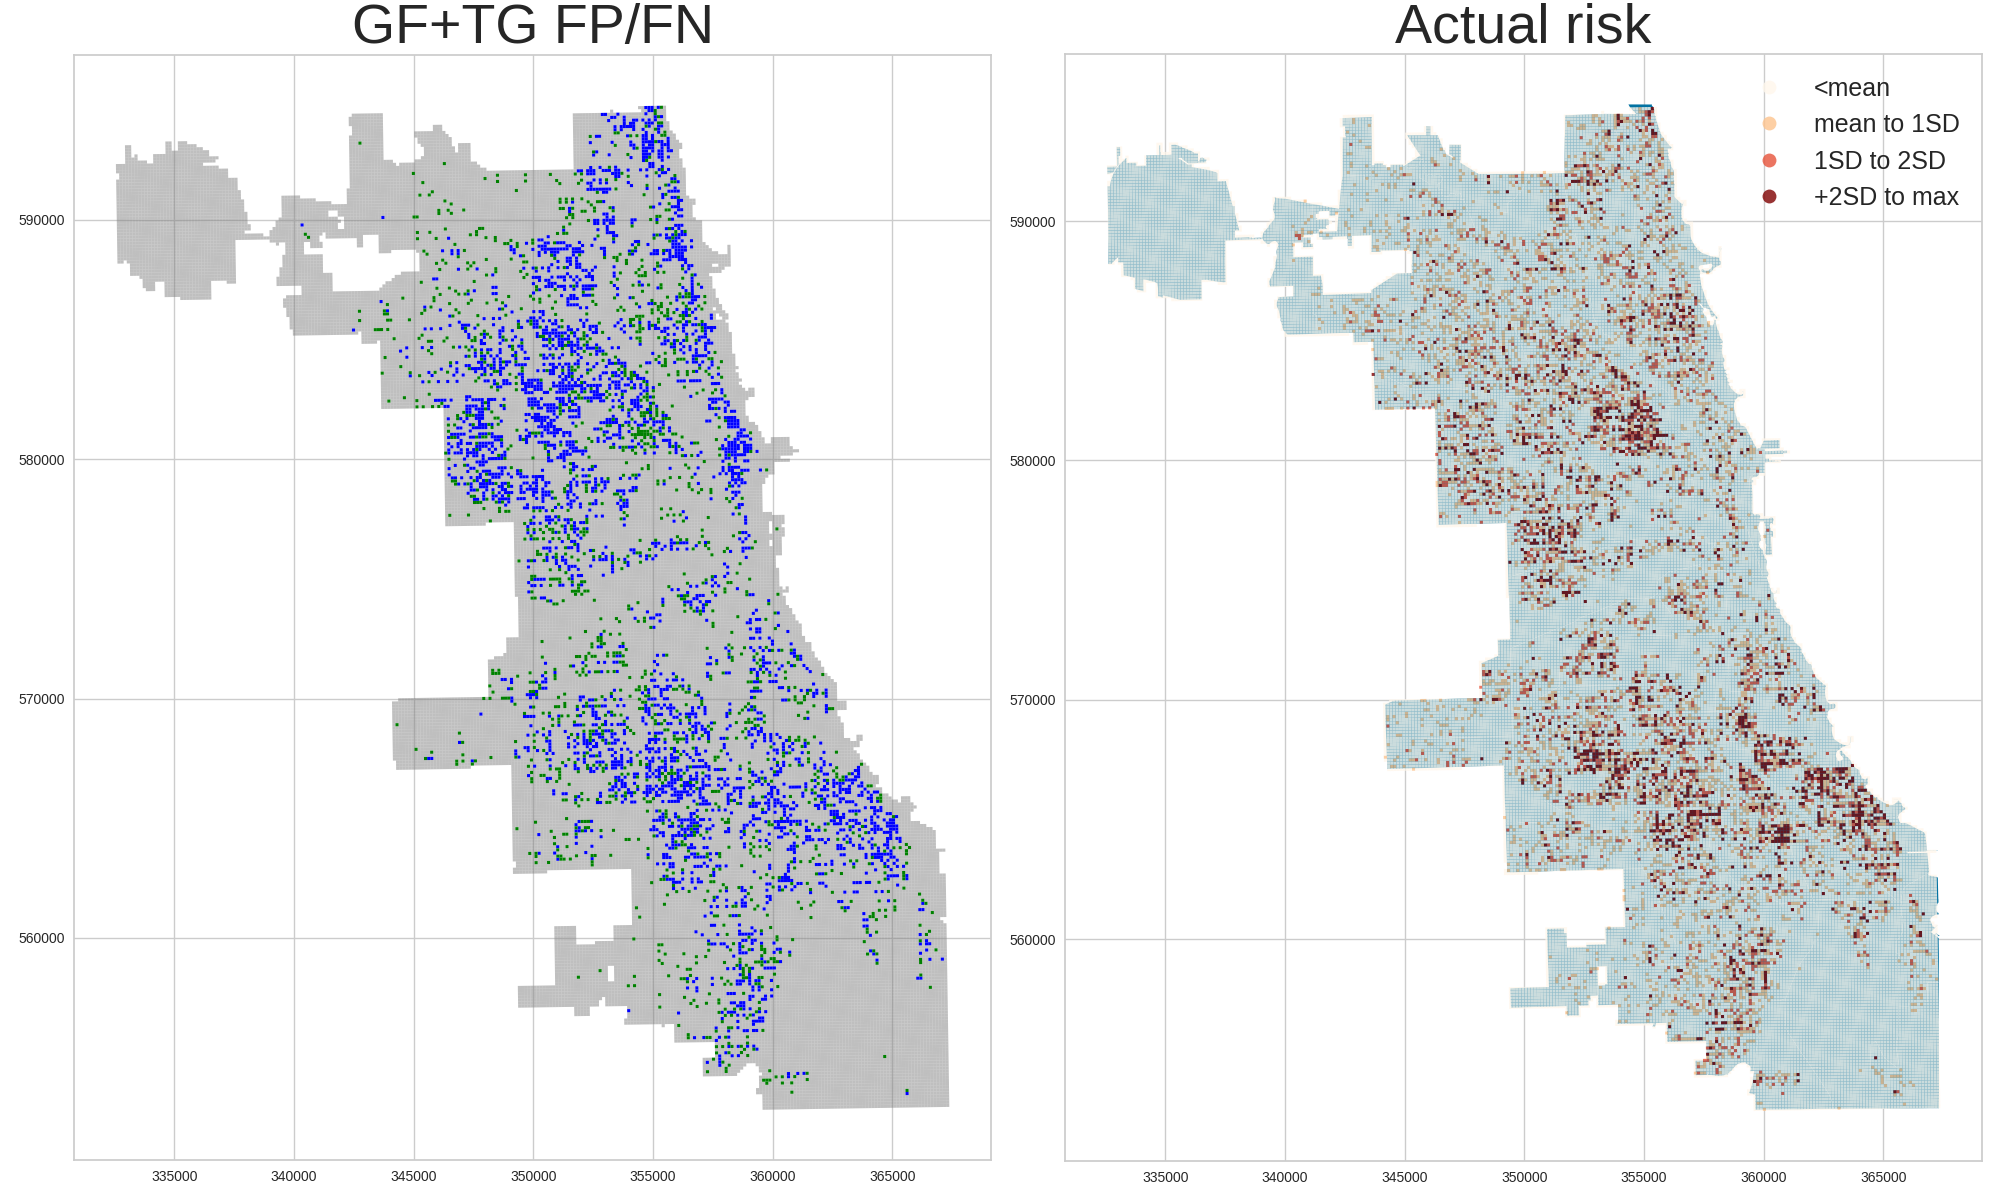
\includegraphics[scale=0.25]{./add-crime-timeseries-fig/GF+TG_fnp.png}
  \caption{左:GF+TGのFPFN 右:実際のリスクマップ}
  \label{fig:add-crime-timeseries-gf-tg-fnp}
\end{figure}
%------------------------------------------
% ROC curve
%------------------------------------------
また,各モデルのROC曲線を図\ref{fig:add-crime-timeseries-roc}に示した.

\begin{figure}
  \centering % 図を中央寄せにする
  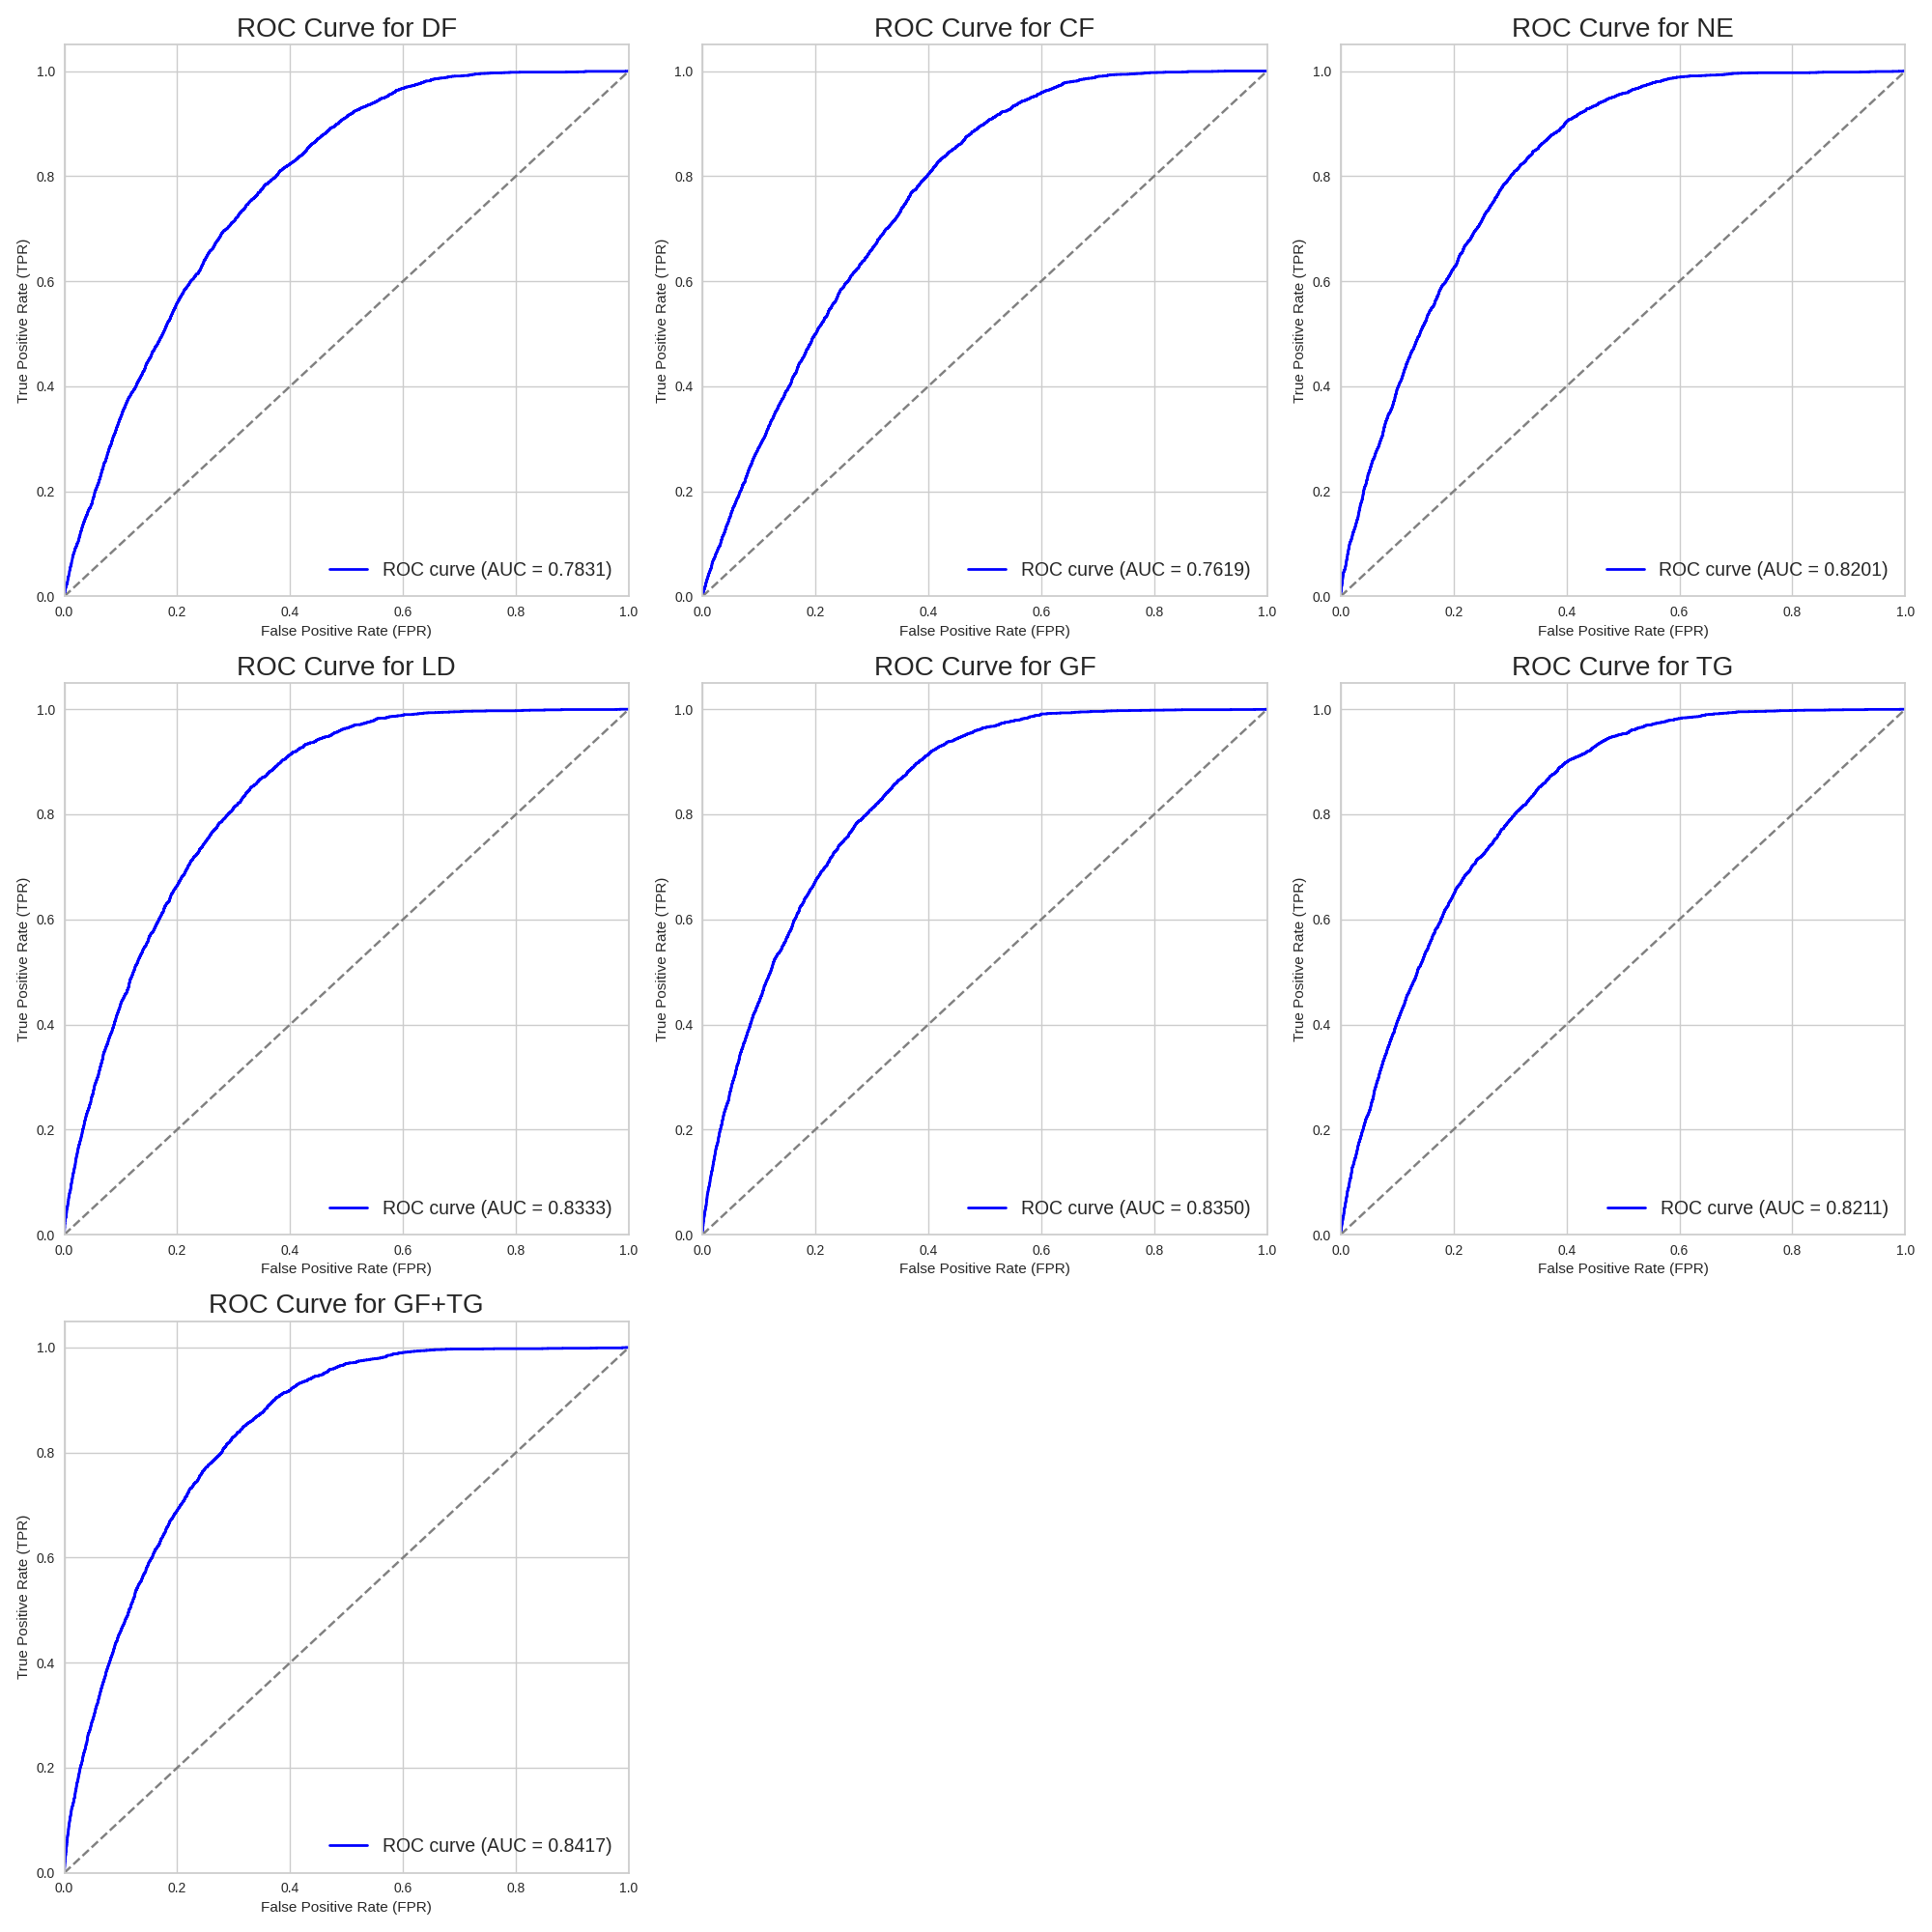
\includegraphics[scale=0.25]{./add-crime-timeseries-fig/roc_auc.png}
  \caption{ROC曲線}
  \label{fig:add-crime-timeseries-roc}
\end{figure}
%------------------------------------------
% table
%------------------------------------------
各モデルの予測精度を精度指標を基に比較した結果を表\ref{tb:fig:add-crime-timeseries-index}にまとめる.
最も的中率が高いモデルはGFであるが,これは偽陽性を評価できていないのでPAIとAUCに注目する.
PAIについて注目すると,DFとCFを比較すると精度が低下したが,
NE,LD,GF,TGでは大きな改善がみられ,
GF+TGが最もPAIが高くなった.
AUCについて注目すると,DFとCFを比較すると精度が低下したが,
NE,LD,GF,TGでは同等の改善が確認され,
PAIと同様にGF+TGが最もAUCが高くなった.

\begin{table}[htbp]
  \centering
  \caption{各モデル間の精度比較}
  \begin{tabular}{l|r||r|r|r|r|r|r}
  \hline

  モデル & DF & CF & NE & LD & GF & TG & GF+TG \\  \hline\hline
  的中率 & 42.6 & 31.3 & 41.9 & 44.3 & \bf{44.6} & 42.5 & 42.9 \\ 
  PAI & 2.38 & 2.29 & 2.80 & 2.99 & 3.04 & 2.79 & \bf{3.14} \\ 
  AUC & 0.78 & 0.76 & 0.82 & 0.83 & 0.83 & 0.82 & \bf{0.84} \\ \hline
  


  \end{tabular}
  \label{tb:fig:add-crime-timeseries-index}
\end{table}

\FloatBarrier